\chapter{Introduction}
\label{c:intro}

\section{Materials science and history}
\label{s:matsci_history}

Metals and alloys are of such importance to humankind that entire eras of our history have been defined by and named after discoveries and advances in metallurgy \cite{metals_prehistory1, metals_prehistory2}. A civilisation's ability to gain mastery of the properties and usage of materials is often strongly correlated with its success in history \cite{metals_success1}. The historical influence of metals and alloys has touched all areas of human existence, from fashion to warfare \cite{metals_social}.

It should come as no surprise that a material's use is often linked to its properties. When a civilisation learned to harness the properties of a novel material, its influence often grew as a result \cite{guns_germs_steel, metals_success2}. Whether building a woodcutter's axe or a fusion reactor, the mechanical properties of materials---metals and alloys in particular---are among the most important considerations for using a material in engineering applications.

Traditionally, such properties have been largely studied via empirical methods such as tensile and compressive tests, beam bending, and indentation \cite{tensile_test_theory, bending_test_theory, indentation_theory}. Such tests have mainly focused on macroscopic scales, thus offering bulk-averaged properties valuable to engineers. Unfortunately, such methods only describe observed behaviours without truly elucidating the fundamental mechanisms behind them \cite{micromech_test1}. Advancing technology has allowed progressively smaller scale tests. Micro- and nano-scale testing, where tests can be performed on carefully controlled samples such as single crystals, thin films, crystal boundaries, etc. For example, it is possible to probe specific slip systems to see how they behave under various loading scenarios \cite{micromech_test2, micromech_test3}. The increased resolution and more thorough parameter control goes a long way in providing a window through which more fundamental behaviours can be observed and hopefully explained; thus providing a way of deconvolving macroscopic observations into their constituent phenomena \cite{micro_macro1, micro_macro2}.

However, understanding the underlying mechanisms behind empirical results through experimental means has proven difficult at every scale \cite{multiscale_model_mats1, multiscale_model_mats2}. Fortunately modelling and simulation can be powerful allies in this task. In particular, the study of dislocations is experimentally challenging \cite{dln_exp_obs1, dln_exp_obs2, dln_exp_obs3}. By virtue of being such an important player in the mechanical properties of materials, dislocations demand careful study from both empirical and in-silico avenues, where insights from one can inform the other, and form a feedback loop that continually advances our understanding.

The story of humanity is the story of our tools. Every leap in technological capability has come as a result of better understanding the materials available to us; from the hand-axes of \textit{homo habilis} to fusion reactors, our increasingly detailed understanding of the properties of materials has enabled us to reach previously unimaginable goals. As we push the boundaries of what is possible, the need for knowledge becomes more important. Progress is made by subjecting our tools to increasingly extreme conditions and working to solve the problems that arise. Some of the most extreme conditions we have ever dreamt of achieving, are those found inside fusion reactors, where radiation damage, large temperature gradients, gas diffusion and plasma instabilities provide the means for properties to change drastically over a components' lifetime \cite{fusmat1, mats_fusion1, mats_fusion2}. In-silico research is an increasingly key component of scientific research. For our purposes, it can aid in the analysis and interpretation of micromechanical tests, as well as provide new fundamental insights that cannot be obtained via traditional methods.

\section{Fusion energy production}
\label{s:fusion}

There currently exist two major branches of research for large scale fusion energy production \cite{icfvsmcf}:
\begin{inparaenum}[\itshape1\upshape)]
    \item magnetic confinement fusion (MCF) \cite{mcf} which confines the plasma using magnetic fields and
    \item inertial confinement fusion (ICF) \cite{icf} which uses a frozen fuel pellet which is either directly or indirectly compressed by arrays of powerful lasers.
\end{inparaenum}
The physics and engineering challenges vary greatly between both approaches but the fundamental materials problems remain largely the same---with a few exceptions such as divertors \cite{icf_mcf1, icf_mcf2}.

\subsection{Operating environment}
\label{ss:operating_env}

A constant feature of nuclear energy production is the exposure of reactor materials to large loads of ionising and non-ionising radiation. In the case of fission, this is mostly in the form of low energy neutrons and residual radiation from fission products. Fusion on the other hand, deals with the sparsely explored 14 MeV neutron spectrum \cite{mats_fis_fus}. The lack of appropriate sources of suitably energetic neutrons \cite{ifmif} has meant that modelling, as well as searching for experimental analogues for the true damage cascades have become a crucial part of materials research \cite{fusmat1s}.

When it comes to fusion, the operating environments change vastly between ICF and MCF, as described by \cref{tab:rad} \cite{openv}. The table should be read with a healthy dose of scepticism, given that the numbers and conditions for commercial reactors, or even reactors capable of producing a net positive amount of energy, are not yet fully known because they do not exist. This is especially true for ICF, where we are \emph{extremely far} from achieving the operating frequencies required for a commercial reactor. However, the table provides a fairly reasonable first approximation of the demands placed on reactor materials for both mainstream types of fusion energy production. That said, the demands on the components needed for energy harvesting---a divertor in the case of MCF, and an open problem for ICF---are conspicuous by their absence.

\begin{table}
    \centering
    \resizebox{\textwidth}{!}{
        \begin{tabular}{llrr}
            \toprule
            Location                         & Radiation Type          & MCF (ITER)                   & ICF (LMJ)                                                                               \\
            \midrule
            1\textsuperscript{st} Wall       & Neutron flux            & \SI{3e18}{m^{-2}.s^{-1}}     & \SI{1.5e25}{m^{-2}.s^{-1}}                                                              \\
                                             & Neutron fluence*        & \SI{3e25}{m^{-2}}            & \SI{3e18}{m^{-2}}                                                                       \\
                                             & $\gamma$-ray dose rate  & \SI{2e3}{\gray.s^{-1}}       & $\sim$ \SI{1e10}{\gray.s^{-1}}                                                          \\
                                             & Energetic ion/atom flux & \SI{5e19}{m^{-2}.s^{1}}      & \ldots                                                                                  \\
            \midrule
            1\textsuperscript{st} Diagnostic & Neutron flux            & \SI{1e17}{m^{-2}.s^{-1}}     & \SI{1e26}{m^{-2}.s^{-1}}                                                                \\
                                             & Neutron damage rate     & \SI{6e-9}{dpa.s^{-1}}        & negligible                                                                              \\
                                             & Neutron fluence*        & \SI{2e24}{m^{-2}}            & $\sim$\SI{1e19}{m^{-2}}                                                                 \\
                                             & Neutron damage          & \SI{1e-1}{dpa}               & negligible                                                                              \\
                                             & $\gamma$-ray dose rate  & $\sim$\SI{1e2}{\gray.s^{-1}} & $\sim$\SI{1e10}{\gray.s^{-1}}                                                           \\
                                             & Energetic ion/atom flux & $\sim$\SI{1e18}{m^{-2}}      & \ldots                                                                                  \\
                                             & Nuclear heating         & \SI{1}{\mega\watt.m^{-3}}    & 0                                                                                       \\
                                             & Operating temperature   & \SI{520}{\kelvin}            & \SI{293}{\kelvin}                                                                       \\
                                             & Atmosphere              & Vacuum                       & Air                                                                                     \\
            \midrule
            Other                            & EM pulse                & \ldots                       & \SIrange[range-units = single]{10}{500}{\kilo\volt.m^{-1}} @ \SI{1}{\giga\hertz}        \\
                                             & Shrapnel                & \ldots                       & \SIrange[range-units = single]{1}{10}{\kilo\metre.s^{-1}} @ $\sim$\SI{30}{\micro\metre} \\
            \bottomrule
        \end{tabular}
    }
    \caption[Estimated operating conditions of MCF and ICF fusion reactors.]{Estimated operating environment comparison between MCF (ITER) and ICF (LMJ). Reproduced from \cite{openv}. Note these numbers are unrepresentative of actual fusion power plants as both ITER and the LMJ are experiments---it is likely power plants will be subject to much harsher operating conditions. \\* End of life.}
    \label{tab:rad}
\end{table}

\Cref{tab:rad} shows that dosages and dosage rates vary wildly between approaches. For the most part, MCF receives higher doses of neutrons and ions in both the first wall and diagnostic equipment. This seems to indicate that the material requirements for MCF are stricter than for ICF. However, shrapnel production is a strong possibility in ICF, especially in indirect drive reactors; where a specially made container called a \emph{hohlraum} holds the fuel pellet and is subsequently obliterated when the pellet undergoes fusion (see \cref{f:hohlraum} \cite{hohlraum}). This is a huge challenge, as such high energy shrapnel would be capable of destroying diagnostic equipment and damaging the first wall \cite{icfpwr1,icfpwr2,icfpwr3}.

\begin{figure}
    \centering
    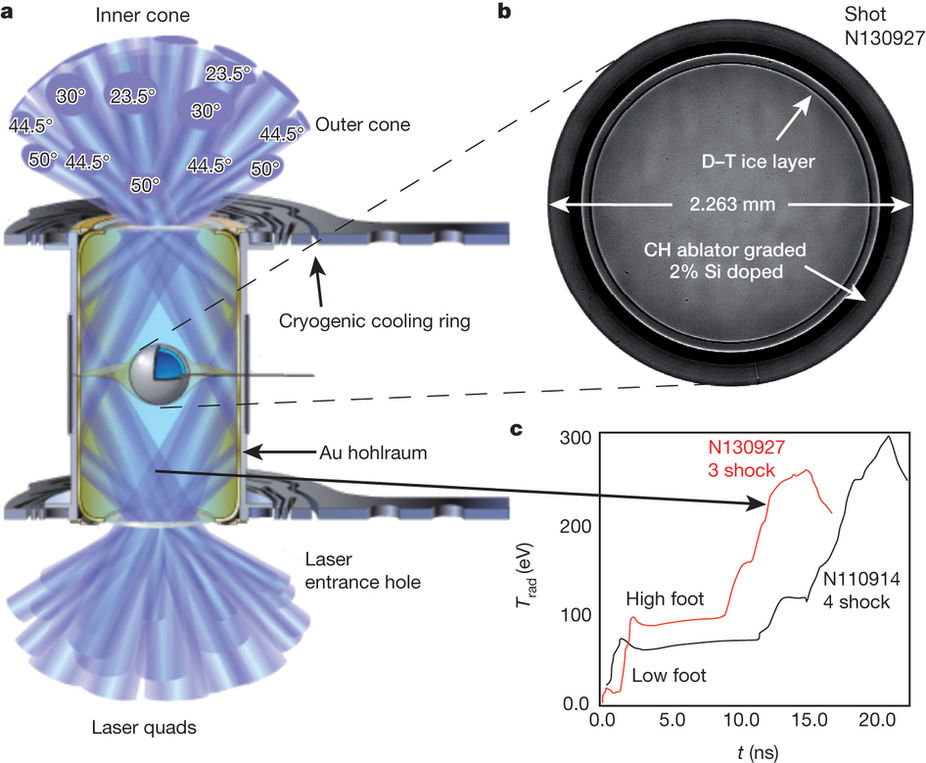
\includegraphics[width=\linewidth]{hohlraum.jpg}
    \caption[Hohlraum design for indirect drive in Inertial Confinement Fusion.]{\textbf{a} Cross-section of the National Ignition Facility's ICF target design showing the gold hohlraum and plastic capsule, fuel pellet, and incident laser bundles. \textbf{b} X-ray image of the actual capsule for N130927 with DT fuel layer and surrounding CH (carbon–hydrogen) plastic ablator. \textbf{c} X-ray radiation drive temperature as a function of time for the National Ignition Campaign (NIC) low-foot implosion and the post-NIC high-foot implosion. Image taken from \cite{hohlraum}.}
    \label{f:hohlraum}
\end{figure}

Overall, the table is unrepresentative of potential operating environments in large-scale power stations, but sets lower limits on the demands of the materials involved in both mainstream proposals for fusion energy production.

\subsection{Effects of radiation on reactor materials}
\label{ss:rad_effect_mat}

\subsubsection{Radiation Damage}
\label{sss:rad_damage}

One of the bigger problems in radiation damage research is the lack of a truly standardised way of measuring damage on materials \cite{srimisbad}. The most common unit is displacements per atom (dpa) \cite{dpa}. It is defined as the average number of displacements undergone by each atom in a material as a result of being irradiated. The fundamental unit of measurement for this, is the number of displacements per unit volume per unit time, $R$
\begin{align}\label{eq:dpa}
    R & = N\int _{E_{\rvar{min}}}^{E_{\rvar{max}}}\int _{T_{\rvar{min}}}^{T_{\rvar{max}}}\phi (E)\,\sigma (E,T)\,\upsilon (T)\;\rvar{d}T\;\rvar{d}E\,,
\end{align}
where $ N $ is the atom number density (no. of atoms per unit volume); $ E $ the incoming particle's energy; $ T $ the energy transferred in a collision of a particle of energy $E$ and a lattice atom; $ \phi(E) $ the energy-dependent particle flux; $ \sigma(E,T) $ the cross-section for the collision of a particle with energy $ E $ resulting in a transfer of energy $ T $ to the struck atom; and $ \upsilon(T) $ the number of displacements per primary knock on atom as a function of transferred energy $ T $. DPA can be calculated by na\"{i}vely multiplying $ R $ by the sample volume and total exposure time (or use fluence, $\Phi(E)$, rather than flux). This ignores the fact that $\sigma (E,T)$ and $\upsilon (T)$ will be locally perturbed in the neighbourhood of damage cascades, but since the bulk volume is much greater than that of the damage cascades', the functions are assumed to remain globally unchanged.

In principle, this is a rather good measure of damage \cite{dpa}. The catch is that, generalised, analytical expressions for $ \sigma(E,T) $ and $ \upsilon(T) $ depend on a slew of parameters and are therefore incredibly hard, if not impossible to derive. That said, they can be discretised and roughly approximated via Monte Carlo (MC) approaches \cite{srim, srimisbad, dpa}. However, damage cascade modelling falls squarely in the realm of pico- to nanosecond timescales, and as such is only tractable with Molecular Dynamics (MD) and Kinetic Monte Carlo (KMC) \cite{dmg_cascade1, dmg_cascade2} approaches. At the end of such cascades, we are often left with dislocation sources or prismatic dislocation loops \cite{dmg_cascade_dln}. Such loops can be used as inputs for Dislocation Dynamics (DD) simulations, which can explore greater temporal and spatial scales \cite{fusmat1s}.

\subsubsection{Transmutation}
\label{sss:transmutation}

Transmutation products are one of the biggest sources of problems for materials in fusion applications \cite{fusmat1, mats_fusion1}. Not only do they tend to embrittle materials, they often also reduce their thermal conductivity \cite{transmute}. The former presents significant challenges for structural materials \cite{ods_rad_res}; the latter is especially egregious for energy extraction by limiting the divertor's ability to conduct heat, thus lowering the reactor's efficiency and causing thermal stresses due to the generation of hot spots that cannot be easily dissipated. As a result, understanding the mechanical and thermal behaviour of transmutation alloys is crucial for moving forward \cite{nirrhard, colcas, hardening}, but doing so requires knowledge of the time evolution of a reactor's components. Since the chemical composition changes in a non-trivial way, so do the mechanical properties. Worse still are the long timescales over which this occurs---on the order of years or tens of years \cite{transmute2}. Even if we were able to experimentally irradiate fusion-relevant materials with appropriately energetic neutrons, it would take years before we could characterise their behaviour, and doing so would be problematic due to radioactive decay.

The way we go about addressing the time-dependent compositional change of a material is to model it. Culham Centre for Fusion Energy's (CCFE), FISPACT \cite{fispact}, takes an MC approach at calculating transmutation and decay products of a sample given certain conditions. The code utilises external data provided by the European Activation File, which provides cross-section and decay rate data for a wide range of isotopes \cite{fispact_library}. Unfortunately, there is a lack of cross-section data for certain neutron energies that contribute in a non-negligible manner to a fusion environment. Interpolating to fill the gaps would not be appropriate as the data is non-smooth and subject to resonance peaks, so the solution is imperfect.

Transmutation products will always be problematic, but they are a fact of working with fusion-relevant materials. Fortunately, there are ways in which inclusions may be modelled via DD (\cref{sss:inclusions}). DD may also be used to model dislocation movement and interaction within heterogeneous media (\cref{ss:multiphase}) as is the case for oxide-dispersion-strengthened (ODS) steels; and transmutation alloys of Tungsten divertors, where Osmium, Rhenium and Tantalum clusters which prove highly problematic for its temperature conductivity and structural integrity \cite{w_cluster1, nirrprop, nirpropmic, nirrmic, ionirrmic, ionirrprop, ionirrprop2}.

\section{Parallel computing}
\label{s:parallel_comp}

Processing chips are made up of millions or even billions of transistors acting as switches in logic gates. Each time a logic gate fires, the capacitors inside them charge and discharge at the chip's frequency otherwise known as clock speed \cite{cpu_trnstor}. Consider the power of any electronic component,
\begin{align}\label{eq:pow_ec}
    P(t) & = I(t) V(t) \,,
\end{align}
where $ I $ is current and $ V $ is voltage, both as functions of time, $t$. The current, $ I $, of a capacitor and the definition of power, $ P $, as functions of time, $ t $, as well as the definition of capacitance are given by,
\begin{align}\label{eq:cap_cur_pow_dt}
    I(t) = C \dfrac{\mathrm{d}V(t)}{\rvar{d}t} \,, \qquad
    P(t) = \dfrac{\rvar{d}E(t)}{\rvar{d}t}\,, \qquad
    C = \dfrac{Q_\rvar{c}}{V_\rvar{c}}
\end{align}
where $ C $ is capacitance, $ E $ the energy stored in the capacitor, $Q_\rvar{c}$ the charge stored in the capacitor and $V_\rvar{c}$ the voltage of the capacitor. Substituting \cref{eq:cap_cur_pow_dt} into \cref{eq:pow_ec} and integrating twice, we obtain the expression for the energy stored in a capacitor,
\begin{subequations}
    \begin{align}\label{eq:e_cap}
        \int\limits_{0}^{E_{c}}\int\limits_{0}^{\infty} \dfrac{\rvar{d}E(t)}{\rvar{d}t}\; \delta t & = C \int\limits_{0}^{V_{c}}\int\limits_{0}^{\infty} V(t) \dfrac{\mathrm{d}V(t)}{\rvar{d}t}\; \delta t\,, \\
        E_{\rvar{c}}                                                                               & = \dfrac{C V_{\rvar{c}}^{2}}{2}  = \dfrac{Q_\rvar{c} V_\rvar{c}}{2} = \dfrac{Q_\rvar{c}^2}{2C}\,,
    \end{align}
\end{subequations}
where $ V_{\rvar{c}} $, $ E_{\rvar{c}} $, $Q_\rvar{c}$ are the voltage, energy and charge stored in the capacitor. Recalling that in a processing chip, the capacitors are charged and discharged at the chip's clock speed $ f $, we arrive at the expression for power consumption, $ P_{\rvar{c}} $, of a capacitor charging and discharging at frequency $ f $ \cite{microelec},
\begin{align}
    P_{\rvar{c}} & = E_{\rvar{c}} f \propto C V_{\rvar{c}}^{2} f \label{eq:p_cap}\,.
\end{align}

Computer chips are rather more complicated, but their power consumption (also known as power dissipation) is described by a simple addition of terms \cite{cpu_pow},
\begin{align}
    P = P_{\rvar{dyn}} + P_{\rvar{sc}} + P_{\rvar{leak}}\,,
\end{align}
where $ P_{\rvar{dyn}} $ is the dynamic power dissipation given by \cref{eq:p_cap}. The two other dissipation mechanisms are:
\begin{inparaenum}[\itshape 1\upshape)]
    \item short-circuit, sc, which depends on frequency and occurs when a direct path from transistor to ground is made as a result of multiple transistors conducting simultaneously; and
    \item leakage, leak, which depends on the voltage and is due to micro-currents between doped parts a transistor.
\end{inparaenum}
Furthermore, higher voltages and frequencies result in higher temperatures, which in turn mean decreased transistor performance and increased capacitance. The overall result is an energy expenditure curve similar to \cref{f:cpu_en_cnvx} \cite{cpu_en_cnvx} for every processor unit.
\begin{figure}[t]
    \centering
    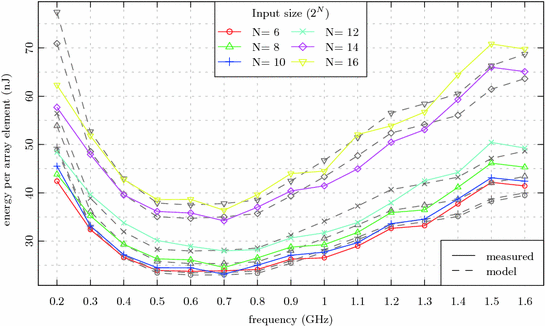
\includegraphics[width=\linewidth]{cpu_en_cnvx.png}
    \caption[Energy expenditure of CPU vs Voltage.]{Energy required by a Samsung Galaxy S2 CPU at \SI{37}{\degreeCelsius} to complete the Gold-Rader implementation of the \emph{bit-reverse} algorithm. The dashed lines denote a theoretical model, image and model found in \cite{cpu_en_cnvx}.}
    \label{f:cpu_en_cnvx}
\end{figure}

This set of optimum conditions is the reason behind the multicore and multithreaded design of modern Central Processing Units (CPUs) and Graphics Processing Units (GPUs). It is also why in recent years there has been such a massive push for parallelism in all computing markets. It is simply not feasible to continually increase clock speeds and voltages because cooling solutions would struggle to remove heat fast enough, and power consumption would skyrocket.

\subsection{Computation on graphics processing units}
\label{sc:compgpu}

\begin{figure}
    \centering
    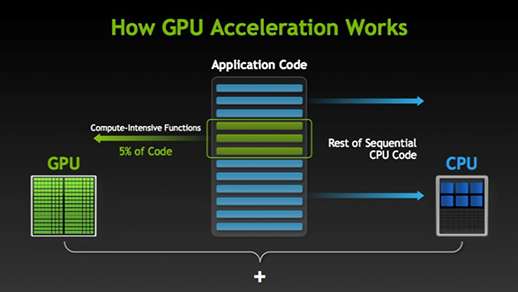
\includegraphics[width=\linewidth]{gpu_parallel.png}
    \caption[CUDA runtime schematic.]{CUDA runtime schematic. Repetitive but computationally intensive tasks can be offloaded to the GPU. Both GPU and CPU are completely indipendent from each other and can work on different parts of the code at the same time, care must be taken to ensure proper syncronisation. Image taken from \cite{nvidia}.}
    \label{f:cuda}
\end{figure}

Central Processing Units (CPUs) are designed not only to perform mathematical operations but logical ones that control program flow. They are tailored to perform the wide variety of operations required by an operating system. These include program scheduling (instruction priorisation, load balancing), instantiation (program loading, unloading, loops, recusion instances) \& branching (if/case statements, go to's), memory operations (fetching, storing, allocation), input/output (IO), and program monitoring (program counters, recursion counters). Modern CPUs have a degree of parallelism and asyncronicity that allows them to increase their total throughput while keeping their operation within near optimal conditions. They are commonly divided into cores and threads, though certain high-end chips have an additional layer named hyperthreading \cite{cpu_arch}.

Given the limited scope of the first computers, the general purpose of CPUs was enough to cover their needs. However, with the advent of personal computers, the demands on CPUs drastically increased. For industrial users these revolved around data acquisition, filtering and preprocessing \cite{fpga, preproc, filtering}. On the other hand, the domestic market demanded ever-increasing levels of abstraction and usability in the form of Graphical User Interfaces (GUIs) such as windows, cursors and sound effects which originally acted as a replacement for haptic feedback. Manufacturers identified this need and moved to provide specialised modules for such tasks. This freed CPU resources and improved user experience by accelerating different processes through hardware means \cite{gpu1, gpu2, gpu3, sound}. These modules include Sound Cards (SCs), Field Programmable Gate Arrays (FPGAs), Graphics Processing Units (GPUs), Application Specific Integrated Circuits (ASICs), Cryptographic Accelerators, Regular Rxpression (RegEx) Accelerators, among others. These external pieces of specialised hardware are collectively dubbed \emph{hardware accelerators}.

Graphics Processing Units were originally intended to offload the very data-intensive but computationally simple operations needed for 3D gaming and rendering \cite{gpu1, gpu2, gpu3}. Graphics processing was a prime candidate for hardware acceleration because the operations on each pixel are largely the same across the screen. Due to their original purpose as gaming and rendering accelerators, they were never designed to operate on higher than single precision data. In fact, single precision (32-bit precision) is still good enough to encode 32-bit colour depth (8-bit channel per RGB colour + 8-bit alpha channel), which only the most high-end monitors support \cite{monitor}. It is also worth noting that because the same operations apply to different pieces of (mostly) independent data, they can all be performed at the same time, often trivially reducing the order of polynomial complexity algorithms. For example, an $\mathcal{O}(N)$ process can be reduced to $\mathcal{O}(1)$ if all $N$ instances fit in a single parallel execution and are independent of one another.

As previously mentioned, GPU parallelism frees up enormous amounts of CPU processing power that can be put to good use running other programs or performing complementary serial processes, while the GPU works concurrently on its dataset. Parallelism has been used by the scientific community for years, but the focus has mainly been on CPU parallelism \cite{cpu_par}. Consequently, its scope was lagerly limited to the use of computational clusters. The two main reasons for this were the fact that GPUs lacked support for higher precision arithmetic, and the very limited to non-existent support for scientific computing in languages such as OpenGL \cite{gpu_comp}.

It wasn't until the development of the OpenCL and OpenACC standards that GPUs caught the attanetion of the scientific community as a viable way of exploiting parallelisation without access to a computing cluster.

OpenCL allows one to work with heteragoenous systems and is similar to C in that it's very low level. It works on a wide range of hardware accelerators and is therefore useful for many scientific and engineering applications, but it's also relatively hard to use. One can make use of libraries written in OpenCL to facilitate development, but it is still a fully fledged C-type language \cite{opencl}.

OpenACC is similar to OpenMP in that they both use pragmas\footnote{Pragmas are especially formated comments that specific compilers recognise and turn into special instructions at compile time. They are not part of the programming language's official standard, but rather compiler-specific extensions. Pragmas are usually programmed in C or Assembly and must be implemented by the compiler manufacturer. Nothing prevents application developers from writing the would-be pragma's code directly into their application, but this can prove a lengthy and difficult process. The rigid nature of pragmas, as well as the compiler manufacturer's priorities, limit their scope and usability.} and they both work in shared memory environments---same GPU and same CPU respectively. This is no coincidence as OpenACC was designed as an extension of OpenMP for developing parallel applications on hardware accelerators. Unfortunately, being pragma based, the standard requires significant work by compiler manufacturers, so its adoption has therefore been slow \cite{openacc}. Furthermore, despite simplifying development and minimising the barrier to entry, the use of pragmas limits the flexibility and adaptability of the framework compared to OpenCL.

Recently however, a third option has become viable. NVidia's Computer Unified Device Architecture (CUDA) framework provides the best aspects of both OpenCL and OpenACC. The tradeoff is that it only works on NVidia GPUs and is a closed source product. However, the accessibility and flexibility of CUDA provides anyone familiar with C/C++ the means to develop a GPU application with little issue. NVidia is also strongly backing scientific research by adding double precision support on their GPUs. They have also worked to provide parallel equivalents of well known serial libraries---such as cuBLAS \& cuFFT---for scientific computing. They have additionally developed a wide range of specialist graphics cards tailor-made for scientific purposes. As such, they are the leaders in GPU computing in scientific communities \cite{nvidia}.

\subsubsection{Hurdles for parallelisation}
\label{sc:hurdpara}

\begin{figure}
    \centering
    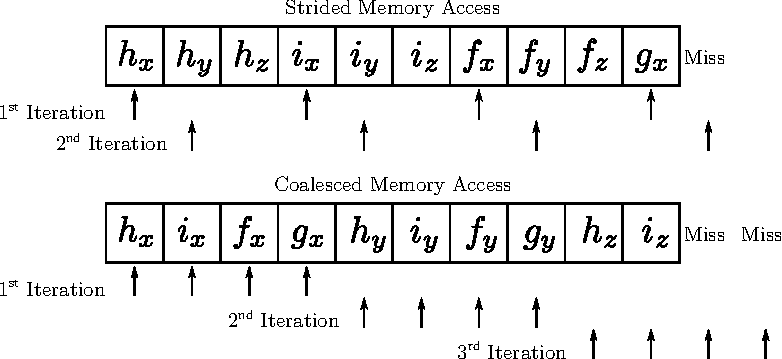
\includegraphics[width=\linewidth]{mem_access.pdf}
    \caption[Memory access pattern example.]{Arrows represent fetch requests by single threads in a GPU. Data should be arranged in such a way that all threads in a warp (collections of 32 threads) can simultaneously access contiguous memory locations, reducing cache-misses and improving throughput. This access pattern can be unintuitive when parallelising serial algorithms, but is extremely important, especially when using scientific computing cards, as they are optimised for long computation times and low memory fetch frequency.}
    \label{f:mem_accessIntro}
\end{figure}

The difficulty in parallelisation varies tremendously from problem to problem. Problems where data is uncorrelated and independent---such as sampling well-behaved probability distributions---are almost trivially parallelisable. Problems where data is correlated or strongly dependent on its neighbours---such as Dislocation Dynamics---require a more careful approach \cite{parallel_algs}.

The largest hurdle when implementing parallel algorithms is often the efficient use of data. In order to obtain good parallel performance, a lot of thought has to be placed on data access patterns, data read/write conflicts, and memory allocation and transfer \cite{nvidia}. For best performance, all this must be analysed on a case by case basis. If done incorrectly, the performance of a parallel application may be lower than the serial version. One must consider a wide range of parameters to successfully parallelise a problem. Among these are GPU architecture, problem size, computational and memory complexity, code branching, required arithmetic precision, and error tolerances \cite{nvidia, gpu_rev}.

Efficient parallelisation of many problems requires \emph{coalesced memory access} as shown in \cref{f:mem_accessIntro}, which means we have to be extremely careful when mapping CPU memory to global GPU (device) memory. The fact that threads work ``simultaneously''\footnote{Not quite but essentially simultaneously. See \cite{nvidia} for details.} means that in order to obtain good performance, data which is to be simultaneously loaded into each thread must be contiguous. This maximises cache memory use and therefore reduces slow memory fetch operations.

Special cases, such as having a parallel dislocation line segment to a surface, as discussed in \cref{ss:analytic_forces}, must be treated carefully due to the way code branching works in GPUs. There are various ways of doing so:
\begin{inparaenum}[\itshape 1\upshape)]
    \item if the special case is inexpensive, it can be treated within the same GPU function;
    \item if the special case is expensive and always known (such as certain boundary conditions in FEM), it can be placed in its own GPU function that treats it separately;
    \item if the special case is expesive and only found at runtime, it may be asynchronously treated by the CPU or buffered into its own GPU function to be executed at a later time.
\end{inparaenum}

\begin{figure}
    \centering
    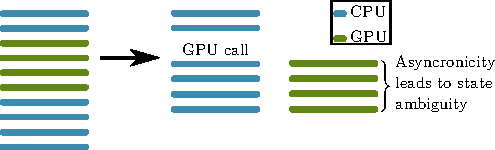
\includegraphics[width=\textwidth]{async.pdf}
    \caption[GPU and CPU asynchronous execution.]{GPU and CPU code run independent of each other. This can lead to state ambiguities if both sides need to be aware of one another \cite{nvidia}.}
    \label{f:async_gpu_cpu}
\end{figure}
One of the advantages of GPU-CPU independence is that both can work concurrently on different aspects of the problem. If both systems have to talk to each other, or there are any race conditions (one process needs to finish before the other can start), then one must tread carefully, ensuring proper syncronisation and data mapping before proceeding (see \cref{f:async_gpu_cpu}).

The reason why code branching is bad for GPU parallelisation is down to the fact that they work like software-customisable vector machines. As in vector processors, collections of threads all carry out the same operation on different pieces of data at the same time. The threads essentially behave as one, operating on different data. This is advantageous to a GPU because it means more energy and space can be used for computation rather than logic and scheduling. However, this eliminates the ability of code to branching within each collection of threads. This means that every branch of an \texttt{if} or \texttt{switch-case} statement will be executed whether a condition is met or not\footnote{If the branch can be resolved at compile time, it is possible for the compiler to prune it as part of compile time optimisation. However, this can be unreliable and depends on how transparent the optimsation is to the compiler, how agressive the optimisation setting is, and how the compiler is implemented. Therefore, relying on compile time optimisation to prune branches is not recommended.}. Only data storage depends on whether a condition is true or false, as illustrated in \cref{f:code_branching}.
\begin{figure}
    \centering
    \begin{subfigure}[t]{0.48\textwidth}
        \centering
        \begin{minted}{c}
if (y == 0){
    x = a+b;
}
else if (y == 1){
    x = a*b;
}
else{
    x = a/b;
}
			\end{minted}
        \caption{CPU code will only execute if the condition is met. This is called code branching.}
    \end{subfigure}
    ~
    \begin{subfigure}[t]{0.48\textwidth}
        \centering
        \begin{minted}{cuda}
p = (y == 0);
p: x = a+b;

p = (y == 1);
p: x = a*b;


!p: x = a/b;
			\end{minted}
        \vspace{12pt}
        \caption{GPU code executes every line but only stores results if the flag before the colon is true.}
    \end{subfigure}
    \caption[Explanation of warp divergence.]{The NVidia CUDA compiler replaces \texttt{if} and \texttt{case} statements with logical flags \texttt{p}. Every line is executed, but the data is only stored if the flag prior to the colon is true \cite{nvidia}. This means that having rare but computationally expensive special cases will tank parallel performance and must therefore be dealt with separately.}
    \label{f:code_branching}
\end{figure}

Dislocation Dynamics (DD)---in particular 3D Discrete Dislocation Dynamics (3D DDD)---can greatly benefit from parallelisation, especially when coupling to Finite Element Methods (FEM). It is worth noting that there are potential issues arising from the very computationally expensive functions and special cases that often arise from analytical solutions in 3D DDD. There are also potential issues with data redundancy---which are non-limiting in the short term---that may eventually require a more data-efficient approach as the computational capabilities and data capabilities of GPUs converge. \Cref{ss:parallel_ddd} expands on these issues in the context of DD.

\section{3D dislocation dynamics modelling}
\label{s:3d_ddd}

The plastic deformation of materials is generally governed by the generation and motion of line defects known as dislocations through the crystal lattice. Microstructural features such as grain boundaries, precipitates and inclusions impede dislocation motion causing strengthening but often limiting ductility \cite{init_fail_dln}. Understanding the behaviour of the dislocation ensemble is highly complicated even when ignoring dislocation-microstructure interactions. However, if we want to truly comprehend their real-world behaviour, we cannot limit ourselves to idealised scenarios.

One of the most often used parametrisations of DD is Discrete Dislocation Dynamics (DDD). Where dislocations are parametrised as a series of nodes linked by straight line segments. This reduces computational requirements and allows for analytic solutions to be obtained. At present, neither DDD nor Finite Element (FE) models can truly handle all the complexities of real-world alloys \cite{ddd_fem1, paradis, fem_ddd2, fem_ddd}. For one, DDD relies on assuming a linear-elastic isotropic solid domain with periodic or infinite boundary conditions, while FE relies on assuming continuum properties inside a \emph{finite} domain.

Crystal Plasticity Finite Element Methods (CPFEM) use constitutive equations to calculate dislocation motion and generation on a set of slip systems. These are given as dislocation densities and thus can still be considered ``bulk'' models because there are no explicit dislocations interacting with one another \cite{cpfem1}. CPFEM can handle finite strains and anisotropy but not strain localisation/slip bands, etc.

Furthermore, dislocations often accumulate in the vicinity of microstructural features. The interaction of dislocations with microstructure and other dislocations can lead to work hardening and local stress concentrations that can lead to failure initiation \cite{size_effects, dln_ind_hard}. Hardware accleration, i.e. using Graphics Processing Units (GPUs), has been shown to be very effective in DDD \cite{gpu_ddd}, and has the potential to enable the simulation of much larger numbers of dislocations for longer timescales. In order to study these phenomena we must find a way of coupling DDD and FEM into a single multiscale model with the potential to simulate micromechanical tests more accurately than CPFEM. With a model such as this, we may potentially be able to predict and observe emergent phenomena/properties, explain michromechanical behaviours, and even predict and explain experimental results based on underlying dislocation mechanisms\footnote{Though predicting and replicating experimental results requires the initial conditions of the experiment and simulation be roughly equivalent.}.

\subsection{Coupling dislocation dynamics to finite element methods}
\label{ss:ddd_fem}

Coupling dislocation dynamics (DD) to FEM is important to properly simulate micromechanical tests because DD provides us with a more precise set of inputs and greater granularity for solving the FE problem. There are at present two methods with which to do so, the \nameref{sss:superposition} and the \nameref{sss:discrete_continuum}. Discrete dislocation dynamics, where the dislocation is broken into nodes connected by segments is a relatively compuationally- and data-efficient implementation of dislocation dynamics, which has the added advantage of having analytical solutions for straight-line segments. However, as discussed in \cref{sss:lvl_set}, explicit discretisation is not the only way to tackle the problem.

\subsubsection{Superposition model}
\label{sss:superposition}

\begin{figure}
    \centering
    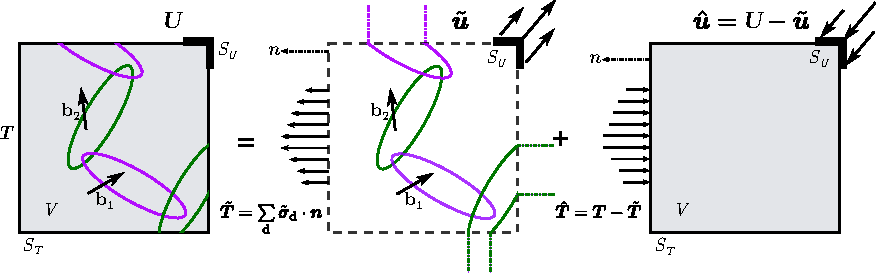
\includegraphics[width=\linewidth]{fem_ddd.pdf}
    \caption[Superposition Model for DDD-FEM coupling.]{The superposition used to couple DDD and FEM. The volume $V$ is bounded by a surface $S = S_{T} \cup S_{U}$ and contains a dislocation ensemble and is subjected to tractions $\vec{T}$ on $S_{T}$ and $\vec{U}$ on $S_{u}$. First, the traction, $\vec{\tilde{T}}$, and displacement, $\vec{\tilde{u}}$, fields due to the dislocations in the infinite domain (DDD) are evaluated on the boundaries $S_{T}$ and $S_{U}$ respectively. Then an elastic boundary value problem can be solved with FEM to calculate the corrective elastic fields required to satisfy the boundary conditions $\vec{\hat{T}} = \vec{T} - \vec{\tilde{T}}$ and $\vec{\hat{u}} = \vec{U} - \vec{\tilde{u}}$.}
    \label{f:fem_ddd}
\end{figure}

The Superposition Model (SM) works by decomposing the problem into separate DDD and FE problems (\cref{f:fem_ddd}). It is assumed that a linear-elastic body $ V $ bounded by a surface $ S $ is subject to traction boundary conditions, $ \vec{T} $, on $ S_{T} $ and displacement boundary conditions, $ \vec{U} $, on $ S_{u} $. The formulation proposed in \cite{dismot} to impose traction-displacement boundary conditions on DDD problems in finite domains states that the total displacement and stress fields can be written as a superposition of displacement and stress fields obtained from DDD and FE,
\begin{subequations}
    \label{eq:superposition}
    \begin{align}
        \vec{U}      & = \vec{\tilde{u}} + \vec{\hat{u}}\,,            \\
        \tns{\sigma} & = \tns{\tilde{\sigma}} + \tns{\hat{\sigma}}\, .
    \end{align}
\end{subequations}
The, (\textasciitilde), fields are those associated with the dislocation in an infinite medium and are obtained by evaluating analytic fields in a DDD simulation. The corrective, (\textasciicircum), fields are those which must be superimposed to ensure the boundary conditions are met. This means that the image fields can be obtained by running a FE simulation with the ``corrected'' displacement and traction fields,
\begin{subequations}
    \begin{align}
        \vec{\hat{u}}                    & = \vec{U} - \vec{\tilde{u}}\,,                                                                                 \\
        \tns{\hat{\sigma}} \cdot \vec{n} & = \vec{\hat{T}} = \vec{T} - \underbrace{\vec{\tilde{T}}}_{\displaystyle{\tns{\tilde{\sigma}}}\cdot \vec{n}}\,,
    \end{align}
\end{subequations}
where $ \vec{n} $ is the outer unit normal vector to $ S $. As a dislocation segment moves closer to the surface, its (\textasciitilde) field diverges and starts causing numerical problems \cite{bdd}. \Cref{ss:paperIntro} is a more in-depth discussion on the superposition method and dislocation-induced surface tractions.

A further problem with this method is that modelling elastic inclusions not only requires the calculation of forces induced by dislocations on the inclusion's surface, but also demands the calculation of so-called polarisation stresses due to differences in the inclusion's and matrix elastic properties \cite{dismot, bdd, ddd_precip}.

That said, the relative simplicity of the superposition method has made it a popular choice \cite{analytic_tractions, ddd_fem_sm, ddd_fem_sm2} for coupling DDD and FEM because all it requires is the calculation of forces and displacements on the boundaries (see \cref{ss:analytic_forces}).

\subsubsection{Discrete continuum model}
\label{sss:discrete_continuum}

The Discrete Continuum Model (DCM) takes an alternative approach to solving the same coupling problem. The DCM only treats short-range dislocation-dislocation interactions analytically while all other interactions are numerically calculated via FEM \cite{dcm}. It is based on the regularisation of the atomic displacement jump across the slip plane into a plastic strain inclusion according to eigenstrain theory \cite{eigenstrain}. Like the Superposition Model, the DCM also assumes the simulated volume to be linear-elastic.

The eigenstrain formalism assumes that material defects can be represented as stress-free strain distributions, dubbed \emph{eigenstrains} \cite{eigenstrain}. For example, a dislocation loop of any shape may be approximately represented by thin, coherent, plate-like inclusions with the same contour as the loop and a characteristic thickness, $ h $, as shown in \cref{f:eigenstrain} \cite{dcm}. The eigenstrain tensor, $ \epsilon^{\rvar{p}} $, can then be defined as a symmetric dyadic product of the Burgers vector, $ \vec{b} $, and slip plane normal $ \vec{n} $,
\begin{align}\label{eq:eigenstrain}
    \tns{\epsilon^{\rvar{p}}} & \equiv \dfrac{1}{2h} (\vec{b} \otimes \vec{n} + \vec{n} \otimes \vec{b})\,.
\end{align}
\Cref{eq:eigenstrain} can be used to calculate approximate elastic fields from the stress-free eigenstrain distribution. The approximation is accurate far from the dislocation core \cite{dln_core}. As we move closer---but still outside the core region---the approximation tends toward the exact discrete dislocation solution as $ h \to 0$. From linear elasticity, the total plastic strain is the sum of the individual plastic strains due to each dislocation segment.
\begin{figure}
    \centering
    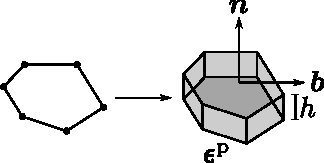
\includegraphics[width=0.5\linewidth]{eigenstrain.pdf}
    \caption[The eigenstrain formalism.]{The eigenstrain formalism as defined in \cite{eigenstrain}. The dislocation is being approximated by a thin coherent inclusion of thickness $ h $, whose strain-free stress tensor $ \tns{\sigma^{\rvar{p}}} $ as defined by \cref{eq:eigenstrain}. The vectors $ \vec{n} $ and $ \vec{b} $ are the normal vector to the slip plane and the dislocation line's Burgers vector.}
    \label{f:eigenstrain}
\end{figure}

The formalism then lets us solve the boundary value problem by finding the stress tensor $ \tns{\sigma} $, elastic strain $ \tns{\epsilon^{\rvar{e}}} $ and displacement $ \vec{u} $ in mechanical equilibrium with the boundary conditions and plastic strain distribution $ \tns{\epsilon^{\rvar{p}}} $ from the ``inclusions''.

It is worth noting that in order to accurately calculate the eigenstrains, there must be sufficient FE nodes inside the thin plate. Therefore, smaller values of $ h $ necessitate finer FE meshes. Furthermore, the original DCM experienced numerical blow up as dislocation-dislocation distances approached $ h $ \cite{dcm0}, but this has since been addressed. Assuming linear-elasticity, the revised model \cite{dcm} yields,
\begin{subequations}\label{eq:discrete_continuum}
    \begin{align}
        \nabla \cdot \tns{\sigma} + \vec{f} = \vec{0} \quad & \in V \setminus \{A\}\,, \\
        \tns{\sigma} = \tns{E} : \tns{\epsilon} \quad       & \in V \setminus \{A\}\,, \\
        [[\vec{u}]] \quad                                   & \rvar{across } \{A\}\,,  \\
        \vec{u} = \vec{u_{0}} \quad                         & \in S_{U}\,,             \\
        \tns{\sigma} \cdot \vec{n} = \vec{T} \quad          & \in S_{T}\,.
    \end{align}
\end{subequations}
At time $ t $, $ \{A\} $ denotes the area swept by the dislocation loops since the start of the simulation. $ [[\vec{u}]] $ denotes displacement jumps tangent to $ \{A\} $ due to dislocation glide; its magnitude and direction depend on the Burgers vector $ \vec{b} $. $ \tns{E} $ is the 4\textsuperscript{th}-order elasticity tensor, $ \tns{\sigma} $ the small strain tensor, $ \vec{f} $ are the body forces and, $ : $, is the double dot product defined as, $ (\tns{E}:\tns{\epsilon})_{ij} = E_{ijkl}\epsilon_{kl} $, between a rank 4 tensor ($ \tns{E} $) and a rank 2 tensor ($ \tns{\epsilon} $). The operator, $ \setminus $, is the set difference defined as, $ A \setminus B = \{x \in A | x \notin B\} $. \Cref{eq:discrete_continuum} can then be linearly decomposed three parts which are solved via FEM or DDD and coupled as described in \cite{dcm}.

It is worth noting that the DCM is \emph{substantially} more complicated than the SM. By requiring the finite elements be small enough for the eigenstate formalism to work, it strongly couples DDD to the FE model and software implementation. It shifts the brunt of the computational workload from DDD to FEM. Essentially trading computationally intensive, long-range interactions which scale on the order of $ \mathcal{O}(N^{2}) $, where $ N $ is the number of dislocation line segments; for computationally intensive tasks scaling on the order of $ \mathcal{O}(M^{3}) $ where $ M $ is the number of finite elements in 3D (assuming linear cubic elements). Furthermore, it cannot be used with BE methods as the eigenstrain formalism demands the use of internal elements rather than simply requiring a surface mesh.

That said, the DCM allows for reductions in the computational complexity of certain parts of the problem which would otherwise have to be done via DDD \cite{dcm}; namely long-range dislocation-dislocation or dislocation-surface interactions via an interaction distance cutoff that is only possible with the eigenstrain formulation. Compared to the superposition method, gains in computational efficiency grow as dislocation density increases with respect to the number of finite elements. Since dislocation-dislocation and dislocation-surface interactions are among the most computationally expensive aspects of DDD, the DCM can reduce the overall computational cost of simulations with large enough dislocation densities and fine enough finite element meshes.

\subsubsection{Level set method}
\label{sss:lvl_set}

Even though the level set method has not strictly been used to couple DD to FEM, it has been used to model inclusions \cite{ddd_inclusion_as_force}, as described in \cref{sss:inclusions}. This type of dislocation dynamics is fundamentally distinct from DDD because Level Set DD uses arbitrary functions rather than a discretisation approach to represent dislocations lines. The idea is that in 3D, a dislocation $ \gamma(t) $ can be represented by the intersection of two zero levels of two level set functions (see \cref{f:lvl_set_dd}),
\begin{subequations}\label{eq:lvl_set}
    \begin{align}
        \phi(x(t),y(t),z(t),t)                                                          & = 0\,, & \qquad
        \psi(x(t),y(t),z(t),t)                                                          & = 0\,,          \\
        \dfrac{\rvar{d} \phi}{\rvar{dt}} = \partial_{t}\phi + \vec{v} \cdot \nabla \phi & = 0\,, & \qquad
        \dfrac{\rvar{d} \psi}{\rvar{dt}} = \partial_{t}\psi + \vec{v} \cdot \nabla \psi & = 0\,,
    \end{align}
\end{subequations}
where $ \vec{v} $ is the dislocation velocity. This definition uses the material derivative because it is assumed that the function and its spatial coordinates are all functions of time, $ t $. The material derivative also comes up when deriving the Navier-Stokes equations of fluid dynamics.
\begin{figure}
    \centering
    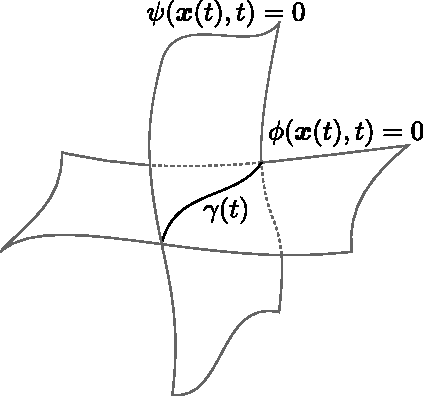
\includegraphics[width=0.3\linewidth]{level_set.pdf}
    \caption[Level set Dislocation Dynamics.]{Diagram of a continuous dislocation $ \gamma(t) $ as the intersection of the zero level of two level set functions $ \phi(\vec{x}(t),t),~\psi(\vec{x}(t),t) $ as posed by \cref{eq:lvl_set}. Image edited from \cite{lvl_set_dd}.}
    \label{f:lvl_set_dd}
\end{figure}

The level set method is significantly more computationally expensive than DDD \cite{lvl_set_dd}. It must solve two coupled quasi-linear partial differential equations whose character is in general undefined. It therefore requires the use of very robust numerical solvers such as higher order Total Variation Deminishing (TVD) Runge-Kutta methods for time discretisation (TVD-RK4 or higher), and high order ENO (Essentially Nonoscillatory $ \mathcal{O}(N^5) $ or higher) or WENO (Weighted Essentially Non-Oscilatory) interpolation methods for spatial discretisation \cite{lvl_set_ddd_inc} for the solutions to converge satisfactorily. The method also makes it impossible to obtain many of the useful analytical solutions one can find by discretising dislocations into straight line segments. Another problem is that this method has never been truly coupled to the finite element method. However, if one were to do so there are two naïve ways of going about it:
\begin{inparaenum}[\itshape1\upshape)]
    \item numerically integrating along the dislocation lines and finding a way to numerically calculate the forces on FE nodes, or
    \item discretising the level set curves and using either the DCM or SM to find forces and displacements.
\end{inparaenum}
The former would be very computationally expensive. Furthermore, no one has found a way to compute the forces or displacements exerted by generally shaped, non-discretised dislocations, numerical solutions are possible as they are needed to find self-interaction energies and dislocation-dislocation forces \cite{lvl_set_dd} but general, closed-form analytical ones are most likely impossible to find. Both approaches defeat the purpose of the level set method, necessitating some form of discretisation whilst keeping the high computational cost. As a result of this, the level set method is not nearly as popular as DDD utilising either the SM or DCM.

\subsection{Non-singular continuum theory of dislocations}
\label{ss:non-singular_dln}

The Peach-Koehler formula describes the fundamental interactions of dislocations \cite{pk_force} according to the force, $ \vec{f} $, that a local stress $ \tns{\sigma} $ exerts on a dislocation line with Burgers vector, $ \vec{b} $, and line direction, $ \vec{\xi} $,
\begin{align}
    \vec{f} & = (\tns{\sigma} \cdot \vec{b}) \times \vec{\xi}\,.
\end{align}

According to \cite{mura_t}, the internal stress field of a dislocation loop in a homogenous, infinite, linear-elastic medium is given by the contour integral around a loop $ L $,
\begin{align}\label{eq:field_stress}
    \sigma_{ij}^{\infty}(\vec{x}) & = C_{ijkl} \oint_{L} \epsilon_{lnh} C_{pqmn} \dfrac{\partial G_{kp}(\vec{x} - \vec{x'})}{\partial x_{q}} b_{m}\; \rvar{d}x'_{h}\,,
\end{align}
where $ C_{ijkl} $ is the elastic stiffness tensor, $ \epsilon_{lnh} $ the permutation operator, $ \vec{b} $ the Burgers vector, and $ G_{kp}(\vec{x} - \vec{x'}) $ is Green's function of elasticity \cite{mura_t}. $ G_{kp}(\vec{x} - \vec{x'}) $ is defined as the displacement component in the $ x_{k} $ direction at point $ \vec{x} $ in response to a unit point force applied in the $ x_{p} $ direction at point $ \vec{x'} $ \cite{a_non-singular_continuum_theory_of_dislocations}. In an isotropic elastic solid, $ G(\vec{x} - \vec{x'}) $, takes the form,
\begin{align}\label{eq:elastic_green_func}
    G_{ij}(\vec{x} - \vec{x'}) & = \dfrac{1}{8\pi \mu}\left[ \delta_{ij} \partial_{pp} - \dfrac{1}{2(1-\nu)} \partial_{ij} \right] R(\vec{x} - \vec{x'})\,,
\end{align}
where $ \mu $, $ \nu $ are the isotropic shear modulus and Poisson's ratio respectively, $ \delta_{ij} $ is the Kronecker Delta, $ \partial_{x_{1} \ldots\, x_{n}} \equiv \dfrac{\partial^{n}}{\partial x_{1} \ldots\, \partial x_{n}}$, and $ R = \lVert \vec{x} - \vec{x'} \rVert $. However, considering that $ \vec{x} \to \vec{x'} \Rightarrow R \to 0 \Rightarrow \partial_{i} R \to \infty $, some (or all) components of the stress field diverge. Furthermore, the total elastic energy also diverges,
\begin{align}\label{eq:e_dln1}
    E & = \dfrac{1}{2} \int S_{ijkl} \sigma_{ij}(\vec{x}) \sigma_{kl}(\vec{x})\; \rvar{d}^{3}\vec{x}\,,
\end{align}
where $ S = C^{-1} $ is the elastic compliance tensor. These divergent properties often prove problematic when numerically computing dislocation forces and energies. \Cref{eq:e_dln1} can also be expressed as a double line integral \cite{dewit1, dewit2},
\begin{align}\label{eq:e_dln2}
    E = & - \dfrac{\mu}{8\pi} \oiint_{L} \partial_{k} \partial_{k} R(\vec{x}-\vec{x}') b_{i} b'_{j} \;\rvar{d}x_{i} \;\rvar{d}x'_{j}\nn
        & - \dfrac{\mu}{4 \pi (1-\nu)} \oiint_{L} \partial_{i} \partial_{j} R(\vec{x}-\vec{x}') b_{i} b'_{j} \;\rvar{d}x_{k} \;\rvar{d}x'_{k}\nn
        & + \dfrac{\mu}{4 \pi (1-\nu)} \oiint_{L} \partial_{k} \partial_{k} R(\vec{x}-\vec{x}') b_{i} b'_{i} \;\rvar{d}x_{j} \;\rvar{d}x'_{j}\nn
        & - \nu \oiint_{L} \partial_{k} \partial_{k} R(\vec{x}-\vec{x}') b_{i} b'_{j} \;\rvar{d}x_{j} \;\rvar{d}x'_{i}\;,
\end{align}
which is important when describing how \citet{a_non-singular_continuum_theory_of_dislocations} derived their non-singular expression.

The singularity in $ R $ is the result of unreasonably and unphysically assuming a dislocation loop's Burgers vector distribution is a Delta function. The assumption was made to allow for closed-form and relatively simple expressions. As noted in \cite{bv_dist}, other distributions may be used but they either result in significantly more complicated expressions or destroy the analytical nature of the classical formulation.

There have been many attempts at removing this singularity, including finite-strain elasticity \cite{non_sing3}, non-local and gradient elasticity \cite{non_sing1, non_sing2}, interaction cut-off radius \cite{pk_force}, average stress at two points on opposite sides of the dislocation line \cite{non_sing4, non_sing5}, and spreading the Burgers vector distribution out over a finite width \cite{bv_dist, non_sing6, non_sing7}. Unfortunately all of these approaches failed in one way or another \cite{a_non-singular_continuum_theory_of_dislocations}. Depending on the approach, various undesirable qualities may present themselves, including
\begin{inparaenum}[\itshape1\upshape)]
    \item inconsistencies with other theories;
    \item impractical implementation;
    \item lack of closed-form solutions for non-straight finite dislocations;
    \item lack of self-consistency; and
    \item the possibility for multiple non-degenerate expressions and solutions for the line integral of the dislocation line energy.
\end{inparaenum}

\Citet{a_non-singular_continuum_theory_of_dislocations} took it upon themselves to define and justify a different Burgers vector distribution that maintains the mathematical convenience of the classical formulation that also eliminates such an unphysical assumption. They did so by introducing a Burgers vector density function,
\begin{subequations}\label{eq:b_dist}
    \begin{align}
        \vec{b}          & = \int \vec{g}(\vec{x}) \;\rvar{d}^{3} \vec{x}\label{seq:bv_dist}\,, \\
        \vec{g}(\vec{x}) & = \vec{b} \tilde{w}(\vec{x}) = \vec{b} \tilde{w}(r)\,,
    \end{align}
\end{subequations}
where $ r \equiv \lVert \vec{x} \rVert $. When substituting \cref{seq:bv_dist} into \cref{eq:field_stress,eq:e_dln2}. The result of multiplying $ R $ with components of $ \vec{b} $ results in the following integrals,
\begin{subequations}\label{eq:r_times_b_dist}
    \begin{align}
        R(\vec{x} - \vec{x}') b_{m}        & = \int R(\vec{x} - \vec{x}'') g_{m}(\vec{x}'' - \vec{x}') \;\rvar{d}^{3}\vec{x}''\,,                                                          \\
        R(\vec{x} - \vec{x}') b_{m} b'_{n} & = \iint R(\vec{x}'' - \vec{x}''') g_{m}(\vec{x} - \vec{x}'') g_{n}(\vec{x}''' - \vec{x}') \;\rvar{d}^{3}\vec{x}'' \;\rvar{d}^{3}\vec{x}'''\,.
    \end{align}
\end{subequations}
Using \cref{eq:b_dist,eq:r_times_b_dist} as guidelines, they defined the following convolutions,
\begin{subequations}
    \begin{align}
        w(\vec{x}) & \equiv \tilde{w}(\vec{x}) * \tilde{w}(\vec{x}) = \int \tilde{w}(\vec{x}-\vec{x}')\tilde{w}(\vec{x}')\; \rvar{d}^{3} \vec{x}'\,, \\
        R_{a}      & \equiv R(\vec{x}) * w(\vec{x}) = \int R(\vec{x} - \vec{x}') w(\vec{x}') \;\rvar{d}^{3} \vec{x}'\,.
    \end{align}
\end{subequations}
At which point they assumed there exists an integrable function $ w(\vec{x}) $ such that
\begin{align}
    R_{a} = \sqrt{R(\vec{x})^{2} + a^{2}} = \sqrt{x^{2} + y^{2} + z^{2} + a^{2}}\,,
\end{align}
where $ a $ is an arbitrary constant meant to represent the dislocation core radius, whose value may be estimated from atomistic simulations. This is essentially a definition that can be used to replace $ R $ in the classical equations and eliminate the singularity by including a free parameter. However, in order to ensure this is mathematically sound, there must indeed exist a function which yields $ R_{a} $ as \citet{a_non-singular_continuum_theory_of_dislocations} defined it. This can be done by making use of the following property for the convolution of two suitably differentiable functions, $ \partial_{i} (f*g) = \partial_{i}f * g = f * \partial_{i} g $. We may take the Laplacian twice,
\begin{subequations}
    \begin{align}
        \nabla^{2}[\nabla^{2} \{R(\vec{x}) * w(\vec{x})\} ] & = \nabla^{2}[\nabla^{2} R_{a}(\vec{x})]\,,                                                             \\
        \nabla^{2}[\nabla^{2} \{R(\vec{x})\}] * w(\vec{x})  & = \nabla^{2}[\nabla^{2} R_{a}(\vec{x})]\,,                                                             \\
        \nabla^{2}[\nabla^{2} \{R(\vec{x})\}]               & = \nabla^{2}\left[\dfrac{2}{R}\right] = -8\pi \delta^{3}(\vec{x}) \label{eq:hand_wavy}\,,              \\
        \nabla^{2}[\nabla^{2} R_{a}(\vec{x})]               & = \nabla^{2}\left[\dfrac{2}{R_{a}} + \dfrac{a^{2}}{R_{a}^{3}}\right] = -\dfrac{15 a^{4}}{R_{a}^{7}}\,, \\
        w(\vec{x})                                          & = \dfrac{15 a^{4}}{8\pi R_{a}^{7}} \label{eq:dist}\,.
    \end{align}
\end{subequations}
\Cref{eq:hand_wavy} is a very brave statement given that,
\begin{align}
    \nabla^{2} \left[R^{-1}\right] & = \nabla^{2}\left[(x^{2} + y^{2} + z^{2})^{-1/2}\right] = 0/\,,
\end{align}
but may be physically justified by pretending $ \nabla^{2}\left[R^{-1}\right] $ arises from assuming a spherical surface of radius 0. \Cref{eq:dist} is a similarly dubious statement that can be justified by noting that,
\begin{align}
    \lim\limits_{a\to 0} w(\vec{x}) = \delta^{3}(\vec{x})\,.
\end{align}
Nevertheless, the non-singular formulation by \citet{a_non-singular_continuum_theory_of_dislocations} fixes the physically and mathematically problematic assumption that Burgers vectors follow 3D Dirac delta distributions, and proves useful in producing analytical expressions (see \cref{ss:analytic_forces}) that are not much more complex than the singular case.

\subsection{Analytical forces exerted by a dislocation line segment on surface elements}
\label{ss:analytic_forces}

Whether using the SM or DCM, coupling DDD to FEM requires the traction field $ \tns{\sigma^{\infty}}(\vec{x}) \cdot \vec{n}(\vec{x}) $ to be distributed among the set of relevant discrete nodes of a FE or BE model. In the DCM model this applies to dislocations that are sufficiently close to the boundary; while in the SM, it applies to all dislocations.
Regardless of the coupling model, the force exerted by a dislocation ensemble on a node $ n $ on element $ e $ is given by,
\begin{align}\label{eq:ddd_fem_force_intro}
    \vec{F}^{(n)} = \int_{S_{e}} \left[\tns{\sigma^{\infty}}(\vec{x}) \cdot \vec{n}(\vec{x})\right] N_{n}(\vec{x})\; \rvar{d}S_{e}\,,
\end{align}
where $ \rvar{d}S_{e} $ is the infinitesimal surface element with surface area $ S_{e} $. $ N_{n}(\vec{x}) $ are so-called shape functions (interpolation functions) that distribute the traction field among the surface element's nodes.

The problematic singularity associated with the classical Volterra dislocation is avoided by using the non-singular formulation of \citet{a_non-singular_continuum_theory_of_dislocations} discussed in \cref{ss:non-singular_dln}, which changes \cref{eq:elastic_green_func} into \cref{eq:ns_elastic_green_func},
\begin{align}\label{eq:ns_elastic_green_func}
    G_{ij}(\vec{x} - \vec{x'}) & = \dfrac{1}{8\pi \mu}\left[ \delta_{ij} \partial_{pp} - \dfrac{1}{2(1-\nu)} \partial_{ij} \right] R_{a}(\vec{x} - \vec{x'})\,.
\end{align}

Using the non-singular definition of $ G(\vec{x}-\vec{x}') $ in \cref{eq:field_stress} we obtain the expression for the stress field of a single straight dislocation line segment bounded by two dislocation nodes at $\vec{x_1}$ and $\vec{x_2}$1, 2) \cite{a_non-singular_continuum_theory_of_dislocations},
\begin{align}
    \label{eq:stressIntro}
    \tns{\tilde{\sigma}}(\vec{x}) = &
    - \dfrac{\mu}{8\pi} \int\limits_{\vec{x_1}}^{\vec{x_2}} \left( \dfrac{2}{R_{a}^{3}} + \dfrac{3a^2}{R_{a}^{5}} \right) \left[ \left(\vec{R} \times \vec{b}\right) \otimes \mathrm{d}\vec{x'} + \mathrm{d}\vec{x'} \otimes \left(\vec{R} \times \vec{b}\right) \right]          \\
    %
                                    & + \dfrac{\mu}{4\pi(1-\nu)} \int\limits_{\vec{x_1}}^{\vec{x_2}} \left( \dfrac{1}{R_{a}^{3}} + \dfrac{3a^2}{R_{a}^{5}} \right) \left[ \left(\vec{R} \times \vec{b}\right) \cdot \mathrm{d}\vec{x'} \right]\vec{I_2}\nonumber                  \\
    %
                                    & -\dfrac{\mu}{4\pi(1-\nu)} \int\limits_{\vec{x_1}}^{\vec{x_2}}  \dfrac{1}{R_{a}^{3}} \left[ \left(\vec{b} \times \mathrm{d}\vec{x'}\right) \otimes \vec{R} + \vec{R} \otimes \left(\vec{b} \times \mathrm{d}\vec{x'}\right) \right]\nonumber \\
    %
                                    & + \dfrac{\mu}{4\pi(1-\nu)} \int\limits_{\vec{x_1}}^{\vec{x_2}} \dfrac{3}{R_{a}^{5}} \left[ \left(\vec{R} \times \vec{b}\right) \cdot \mathrm{d}\vec{x'} \right]\vec{R}\otimes\vec{R}\nonumber,
\end{align}
where,
\begin{align}
    \vec{R}            & = \vec{x} - \vec{x'} = y \vec{l} + r \vec{p} + s \vec{q} \\
    %
    R_a                & = \sqrt{\vec{R} \cdot \vec{R} + a^2}                     \\
    %
    \mathrm{d}\vec{x'} & = -\mathrm{d} y \vec{l}\,.
\end{align}
The vectors $\vec{p}$ and $\vec{q}$ are aligned with the edges of the rectangular finite element, $\vec{n} = \vec{p} \times \vec{q}$ is the element surface normal (pointing away from the dislocation), and $\vec{l}$ is parallel to the dislocation line segment as shown in \cref{f:force_lin_rect}. Then (provided $\vec{l}$ is not parallel to $\vec{p}$ or $\vec{q}$) $\vec{R}$ can be expressed in terms of $(\vec{l},~\vec{p},~\vec{q})$ with coefficients,
\begin{align}
    y = \dfrac{\vec{R}\cdot \vec{n}}{\vec{l}\cdot \vec{n}} \label{eq:problemIntro},\quad
    %
    r = \dfrac{\vec{R}\cdot (\vec{q} \times \vec{l})}{\vec{p}\cdot (\vec{q} \times \vec{l})}, \quad
    %
    s = \dfrac{\vec{R}\cdot (\vec{p} \times \vec{l})}{\vec{q}\cdot (\vec{p} \times \vec{l})}\,.
\end{align}
\Cref{eq:stressIntro} can be turned into a series of triple integrals solved via recursion relations and a few seed functions.

\Cref{f:force_lin_rectIntro} diagramatically summarises the over 40 triple line integrals needed to find an analytical expression of the nodal forces on linear rectangular elements.
\begin{figure}
    \centering
    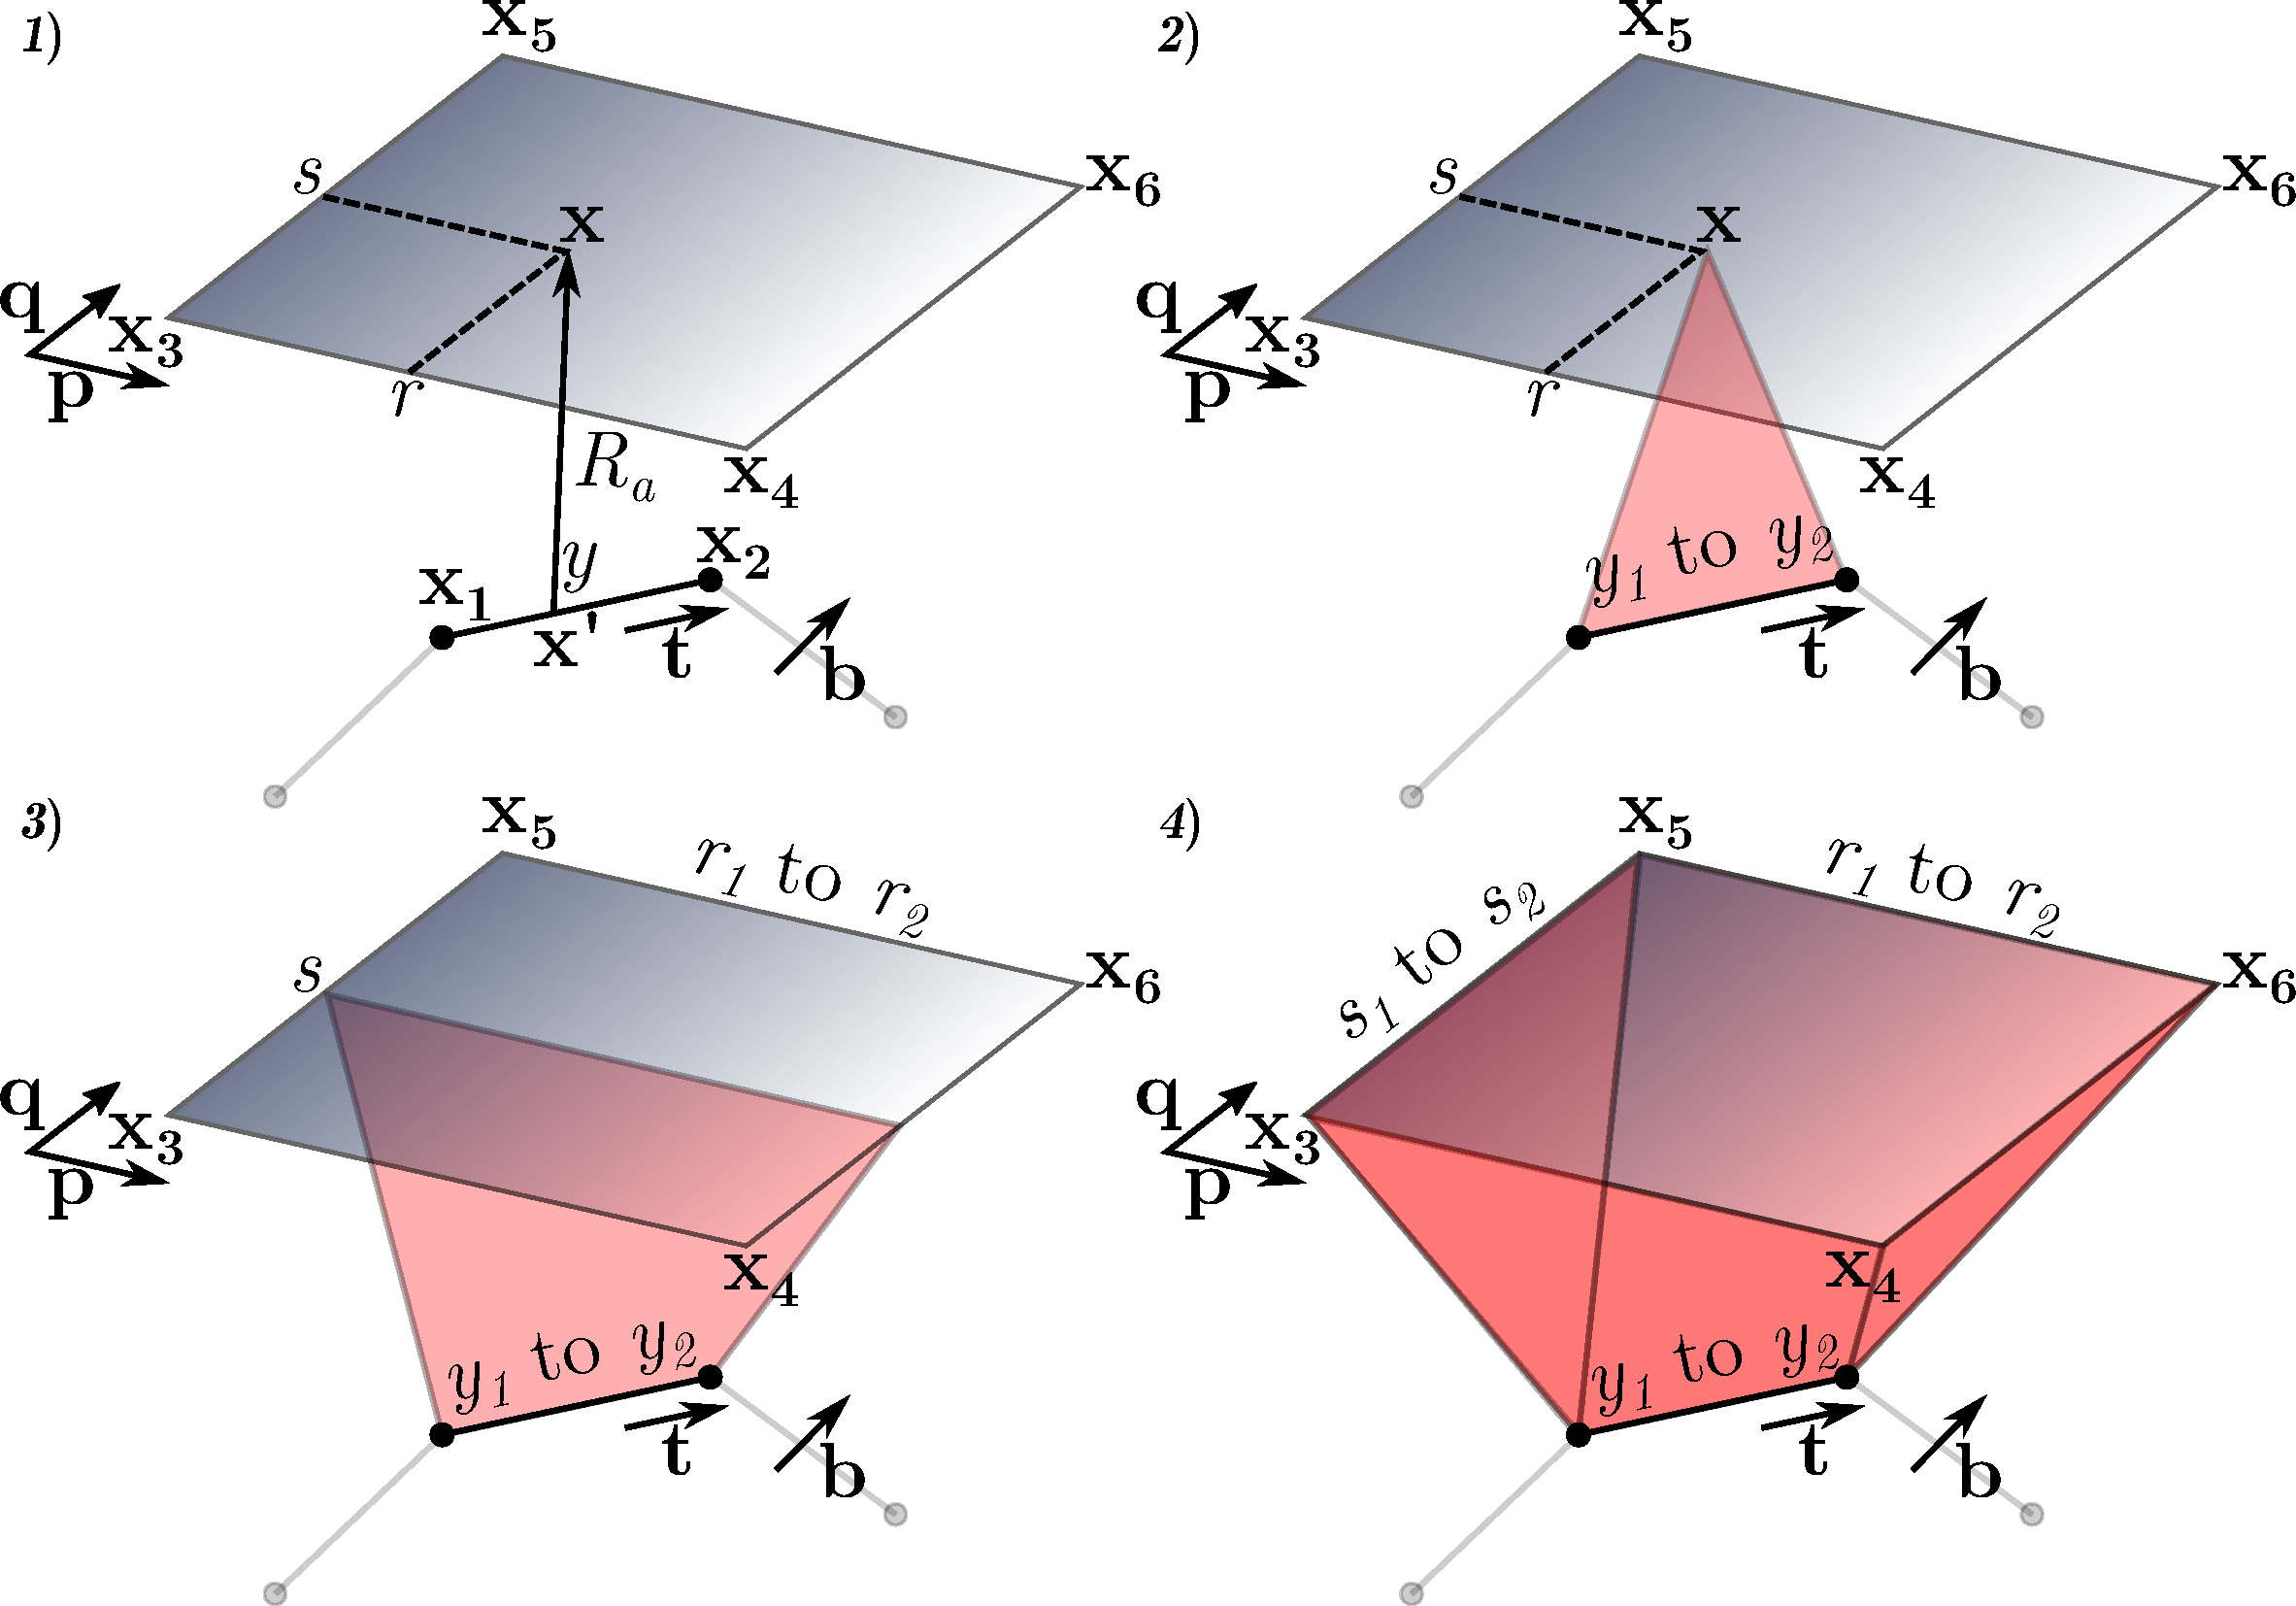
\includegraphics[width=0.8\linewidth]{force_calc_linear_rectangle.pdf}
    \caption[Analytic tractions on linear rectangular surface elements.]{Diagram of the parametric line integrals solved by \citet{analytic_tractions} to find the forces on linear rectangular surface elements.}
    \label{f:force_lin_rectIntro}
\end{figure}
\Cref{c:tractions} contains more detail regarding the theory, implementation and advantages of these analytic tractions over the traditional solution of using Gauss quadrature.

\subsection{Multiphase simulations}
\label{ss:multiphase}

Modelling heterogeneity in DDD remains challenging. The core assumption of DDD is that we have a homogenous linear elastic space with invariant properties. However, modelling multiphase systems such as multicrystals and inclusions necessitates a weakening of such assumptions, particularly the space's homogeneity. Multiphase models are also necessary to apply DDD to more realistic scenarios.

Fusion in particular is riddled with examples of highly heterogenous materials. As previously mentioned, neutron bombardment often causes clustering of transmutation products, particularly on divertor and first wall materials; such clusters often substantially change many of their mechanical and thermal properties. The whole point of Oxide-Dispersion Strengthened (ODS) steels \cite{ddd_ods} is to hamper radiation damage by distributing oxide inclusions within their matrix; if we hope to model such alloys with DDD we must find a way to relax our homogeneity criteria.

Furthermore, many potential candidates for structural and even first wall materials of fusion reactors are designed with complex microstructures in order to resist thermal creep and radiation damage. Understanding dislocation behaviours near the crystal boundaries of these microstructurally complex materials is another niche where DDD simulations can shed light into the mechanisms that give rise to these materials' desirable properties.

\subsubsection{Polycrystalline materials}
\label{ss:polycrystal}

Polycrystalline materials have been studied using DDD, however most of these are in 2D. One of the easiest phenomena to investigate with 2D DDD are grain size effects \cite{2d_pcm, 2d_pcm2}.

It is well known that much of the grain size strengthening effects arise from dislocation-grain boundary (GB) interactions including transmission, reflection, emission and absorption of dislocations \cite{grain_size_eff1, grain_size_eff2}; with transmission being the most typically observed.

These models depend on the grain boundary energy density, $ E_{\rvar{GB}}(\delta\theta) $, where $ \delta\theta $ is the crystallographic misorientation between neighbouring crystals; resolved shear stress, $ \tau $, on the incoming dislocation with Burgers vector $ \vec{b_{1}} $; critical penetration stress for the GB, $ \tau_{\rvar{GB}} $; and Burgers vector of the dislocation debris, $ \vec{\Delta b} = \vec{b_{1}} - \vec{b_{2}} $, left behind when the incoming dislocation, $ \vec{b_{1}} $, transmits throught the grain boundary to become a dislocation with Burgers vector, $ \vec{b_{2}} $. The relationship may be approximated by,
\begin{align}\label{eq:dln_trns}
    \tau \lvert\vec{b_{1}}\rvert^{2} & \geq \tau_{\rvar{pass}} \lvert\vec{b_{1}}\rvert^{2} = E_{\rvar{GB}}(\theta) \lvert\vec{b_{1}}\rvert + \alpha G \lvert\vec{\Delta b}\rvert^{2}\,,
\end{align}
where $ \alpha $ is the material constant and $ G $ the shear modulus. The grain boundary energy density was proposed by \citet{gb_e_dens} to have the simple form,
\begin{align}
    E_{\rvar{GB}} & = 	\begin{cases}
        k \dfrac{\delta\theta}{\theta_{1}}                 & \quad 0 \leq \delta\theta < \theta_{1}\,,          \\
        k                                                  & \quad \theta_{1} \leq \delta\theta < \theta_{2}\,, \\
        k \dfrac{\pi/2 - \delta\theta}{\pi/2 - \theta_{2}} & \quad \theta_{2} \leq \delta\theta < \pi/2\,,
    \end{cases}
\end{align}
where $ k,~ \theta_{1},~\theta_{2} $, are material specific.

This is of course a gross simplification of the real 3D problem, but this approach was used by \citet{2d_pcm} to investigate the Hall-Petch effect, which correlates grain size with flow stress of a polycrystal,
\begin{align}\label{eq:hall_petch}
    \sigma & = \sigma_{0} + \kappa \left(\dfrac{d_{0}}{d}\right)^{n}\,,
\end{align}
where $ \sigma_{0} $ is the yield stress, $ d_{0} $ a reference crystal size, $ \kappa $ the Hall-Petch slope and $ n $ the crystal size sensitivity parameter. \Citet{2d_pcm} showed that the model reproduces the Hall-Petch effect quite successfully. As a consequence, they showed that even what might appear as an overly simplistic approach can describe a complex emergent phenomenon such as the Hall-Petch effect.

Aside from the Hall-Petch effect, the model has also been utilised by \citet{2d_pcm2} to study the thickness effects of three different types of polycrystalline thin films:
\begin{inparaenum}[\itshape 1\upshape )]
    \item no surface treatment,
    \item surface passivation layer, and
    \item surface grain refinement zones.
\end{inparaenum}
In their study, Frank-Reed sources were seeded across the domain, and the superposition principle was utilised to calculate displacement, strain and stresses in the thin films. Their results qualitatively reproduced experimental observations from expected dislocation patterns, stress distributions, and the eventual disappearance of the size effect as the films got thicker.

Though two-dimensional models might seem useless, they have their place, particularly when thin films are concerned. However, they may also be of use when investigating the effects of dislocations on the mechanical behaviour of superconducting tape---whose applications range from medical imaging to fusion energy production. The exotic composition and crystallography of many superconductors (perovskites) would make 3D models very complex and computationally expensive, so 2D models may offer viable alternatives. On top of this, a superconducting tape's operating environment would often have it under strains which might not strictly lie in-plane, but given a small enough segment of tape, strains orthogonal to its plane may be neglected. Thus making 2D models an acceptable first attempt at tacking the problem, at least until developments in 3D models make more realistic studies of such complex systems possible.

The 3D case is substantially more complicated than the 2D case. A study by \citet{twinning}, looked at the role of twinning on the hardening response of polycrystalline Mg using 3D DDD. The article is a perfect example of why 3D DDD is so much more complex than 2D DDD. Admitedly, it uses a material with a HCP crystal structure, whose mobility laws are substantially more complex than those of FCC or BCC materials.

In 3D DDD one must account for dislocation-twin boundary (TB) interactions. These may be obtained via geometric considerations, MD, and experimental evidence \cite{twinning2,twinning3,twinning4,twinning5}. We must have information regarding how dislocations are transmitted through a TB such as
\begin{inparaenum}[\itshape 1\upshape)]
    \item whether a dislocation leaves a residual dislocation on the TB,
    \item the possible pre-TB and post-TB slip planes a dislocation can be transmitted to,
    \item which loading conditions are conducive to which transmission behaviour and
    \item which types of dislocation can be transmitted or reflected and in what ways \cite{twinning}.
\end{inparaenum}
All this obviously depends on the twinning plane, so in order to study more realistic scenarios one must have all the necessary knowledge to properly account for all dislocation-TB interactions. Furthermore, it is possible that certain dislocations may leave behind twinning dislocations that end up as TB steps, whose movement can lead to TB migration and twin growth \cite{twinning6, twinning7}.

\Citet{twinning} modelled four scenarios in order to deconvolve the effects that twins and grain boundaries have on the mechanical behaviour of a cube-shaped crystal. They modelled
\begin{inparaenum}[\itshape 1\upshape)]
    \item a twinned polycrystal with two TBs and GBs on the edges of the cube,
    \item a single crystal with no TBs or GBs,
    \item a polycrystal with no TBs but GBs,
    \item a twinned crystal with TBs but not GBs.
\end{inparaenum}
It is worth noting that the effects of twin growth in plasticity were not accounted for in their DDD simulation and instead had to be numerically computed via the hardening rate $ \theta $,
\begin{subequations}
    \begin{align}
        \theta             & = \dfrac{\rvar{d}\sigma}{\rvar{d}\epsilon} = \dfrac{\rvar{d}}{\rvar{d}\epsilon}  \left[E\left(\epsilon - \epsilon_{\rvar{slip}}^{\rvar{p}} - \epsilon_{\rvar{twin}}^{\rvar{p}}\right)\right] = \theta_{\rvar{s}} + \theta_{\rvar{TG}}\,, \\
        \theta_{\rvar{TG}} & = -\dfrac{\rvar{d}}{\rvar{d}\epsilon} \left[E \epsilon_{\rvar{twin}}^{\rvar{p}} \right] = -E \bar{m} \gamma_{\rvar{twin}} \dfrac{\rvar{d}}{\rvar{d} \epsilon} \left[f_{\rvar{twin}}\right]\label{seq:tg}\,,
    \end{align}
\end{subequations}
where $ \theta_{\rvar{TG}} $ is the hardening rate due to twin growth, $ \bar{m} $ the mean Schmid factor of the participating twins $ \gamma_{\rvar{twin}} $ the characteristic twinning shear and $ \dfrac{\rvar{d}}{\rvar{d} \epsilon} \left[f_{\rvar{twin}}\right] $ is the rate of change of the twin volume fraction with respect to the applied strain. These parameters must be empirically obtained.

With their model, \citet{twinning} managed to qualitatively reproduce experimental observations, including the concave shape of strain-stress curves that arises from the competing hardening effect of TBs restricting dislocation motion (\cref{f:twinning}), and the softening produced by twin growth as obtained from \cref{seq:tg}.
\begin{figure}[t]
    \centering
    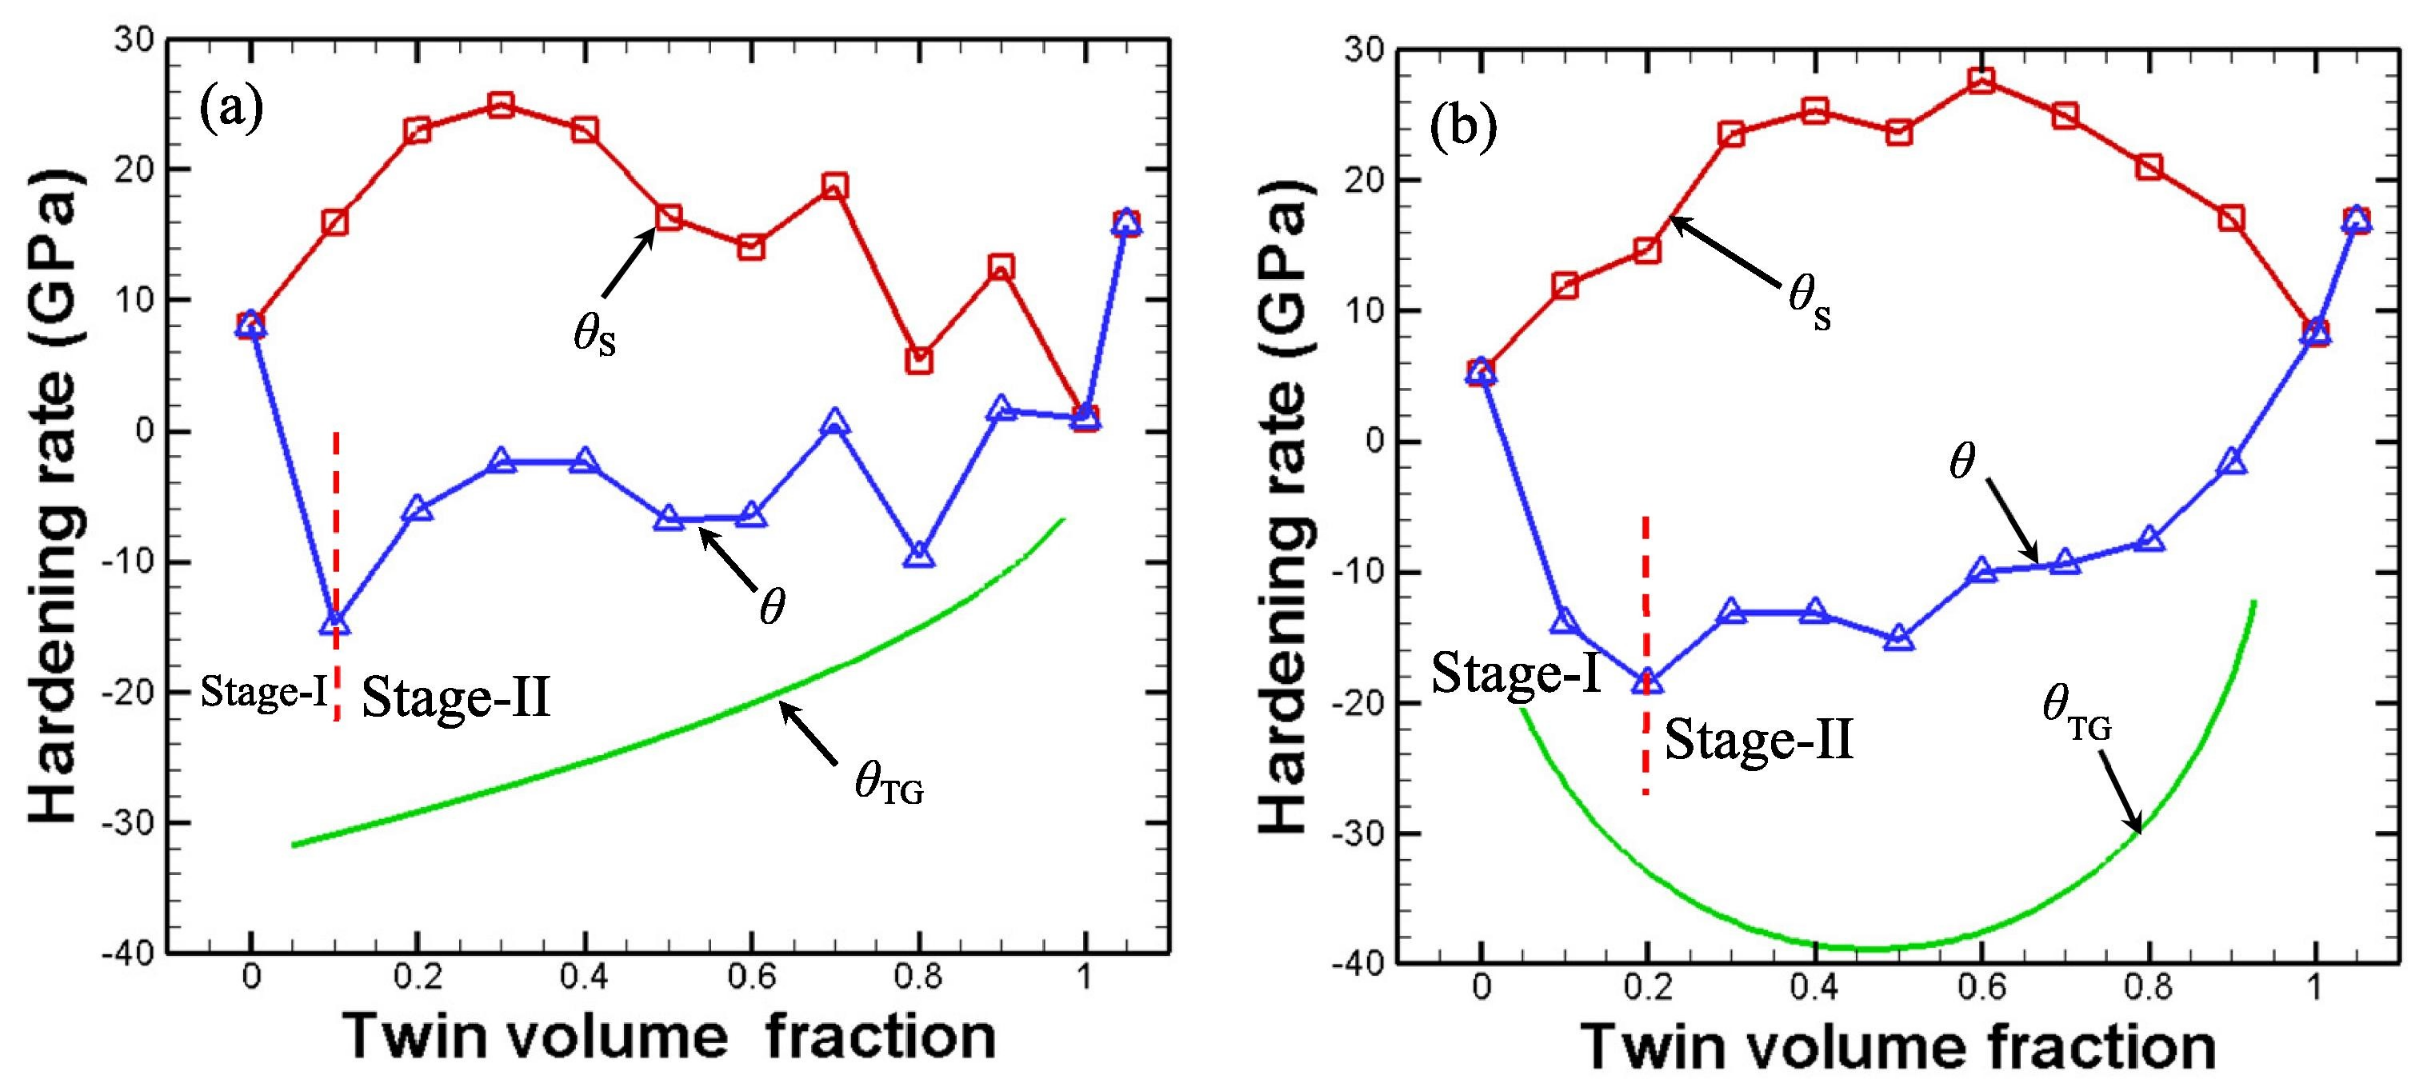
\includegraphics[width=\linewidth]{twinning.png}
    \caption[Modelling twinned multicrystals with DDD.]{Simulated hardening rate as a function of twin volume fraction for (a) yz compressive loading and (b) tensile loading. Image edited from \cite{twinning}.}
    \label{f:twinning}
\end{figure}

Twin boundaries in 3D are analogous to grain boundaries in 2D, given that they are coherent, narrow boundaries rather than messy, often incoherent grain boundaries. Consequently, grain boundaries are much harder to treat in 3D; instead, the community focuses on multiphase models where the details of dislocation transmission between phases are ignored or simplified as expanded upon in \cref{sss:inclusions}.

\subsubsection{Inclusions}
\label{sss:inclusions}

Dislocation-permeable inclusions have been simulated via the SM \cite{sm_incl}. As mentioned in \cref{sss:superposition}, there is a need to calculate polarisation stresses due to differences in the elasticity of both phases. Using the same notation as \cref{sss:superposition} this can be done by breaking up the image stress into,
\begin{subequations}
    \begin{align}\label{eq:sm_pol_stress}
        \tns{\hat{\sigma}} & = \tns{^{\rvar{m}}C} \tns{\hat{\epsilon}} \quad \in V_{\rvar{m}}                                                                                  \\
        \tns{\hat{\sigma}} & = \tns{^{\rvar{p}}C} \tns{\hat{\epsilon}} + \left[\tns{^{\rvar{p}}C} - \tns{^{\rvar{m}}C}\right] \tns{\tilde{\epsilon}} \quad \in V_{\rvar{p}}\,,
    \end{align}
\end{subequations}
where $ \rvar{m},~\rvar{p} $ denote whether a variable belongs to the matrix or precipitate respectively and $ \tns{C} $ is the elastic stiffness tensor.

\Citet{sm_incl} not only modelled a cuboid inclusion, but bimetallic interfaces in 3D. They found that under the right conditions, dislocations can pass from one phase to the other. When a dislocation passes into a different phase, it leaves an antiphase boundary on the slip plane. Therefore, in order for a dislocation to move from one phase to another, it needs excess energy equal to the antiphase boundary (APB) energy of the area it sweeps within the precipitate. This means that as a node passes from one phase to another, it feels a repulsive force $ F_{b} $. The next dislocation moving along the same APB will then feel an attractive force, $ F_{b} $ to dissolve the APB. Once both dislocations move into the new matrix, they form a superdislocation bound by the APB energy \cite{apb}. However, as the dislocation length increases with respect to the precipitate's volume, the production of Orowan loops around it becomes more energetically favourable than moving into the new phase \cite{sm_incl, apb}. Both of these behaviours have been observed when using the superposition method.

The eigenstrain method \cite{eigenstrain_incl} as described in \cref{sss:discrete_continuum} has been shown to be a viable solution to this problem. One can compute the stresses and displacements produced by the dislocation ensemble on the inclusions' surfaces via DCM or SM. The SM method however needs to calculate polarisation stresses \cite{bdd}, an operation that significantly increases the number of calculations necessary to solve the problem.

The DCM method has been used to simulate multiphase materials where the simulated dislocations reproduced experimentally observed behaviours such as the zig-zag patterns and dislocation forests produced by dislocations around precipitates in nickel superalloys \cite{dcm0, dcm_incl}. Reproducing such behaviours is not as trivial as simply adding inclusions to the simulation domain. In order to produce accurate results, one requires knowledge of the coherency stress between the different phases \cite{dcm_incl}. Such stresses are often due to lattice mismatches and differences in the thermal expansion coefficients. These coherency stresses localise the dislocations around the inclusions and are responsible for the observed localisation and aggregation of dislocations around precipitates as seen in \cref{f:coherency} \cite{dcm_incl}.
\begin{figure}[t]
    \centering
    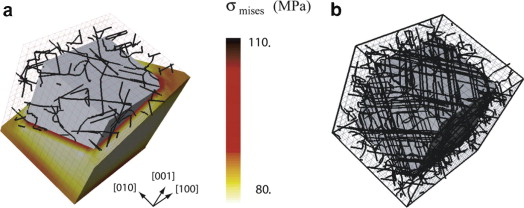
\includegraphics[width=\linewidth]{dln_inclusion.jpg}
    \caption[Modelling dislocation inclusion interactions with the discrete continuum model.]{(a) Shows the initial dislocation configuration after relaxation in the presence of the calculated von Mises coherency stresses $ \tns{\sigma}_{\rvar{mises}} $. (b) Shows the dislocation forresting around the inclusion as a result of 0.2\% plastic strain for the [001] case. Image obtained from \cite{dcm_incl}.}
    \label{f:coherency}
\end{figure}

The level set method has also been successfully used to model inclusions. In contrast to the aforementioned methods, they are assumed to be regions in space where dislocations experience a repelling force, instead of a region in space with distinct characteristics to the matrix. The force profile can be very simply defined to depend on the radial distance from the dislocation to a point in the ``inclusion's'' volume \cite{ddd_inclusion_as_force}. It can also be modulated depending on the nature of the inclusion by making the force a radial function, thus avoiding many of the numerical issues facing DDD-FEM couplings (see \cref{ss:ddd_fem,ss:analytic_forces}). It is also possible to make the inclusions impermeable or semi-permeable depending on the magnitude and steepness of the force gradient, as presented in \cite{ddd_inclusion_as_force}. Arbitrarily shaped inclusions are also possible if one were to also use angular components in the force function, through the use of spherical harmonics and even piecewise-parametric fourier series. This is a simple and versatile method that can be applied to DDD as well.

Though mathematically appealing, such an approach is far from representing the reality of dislocation-inclusion interactions. More realistic scenarios require the use of more commonplace DDD-FEM coupling methods. Implementing arbitrarily-shaped particles is not impossible in DDD---particularly if they can be discretised. Aside from the significantly lower computational requirements of the time evolution and dislocation-dislocation interactions compared to the level set method, one of the biggest advantages of using the SM and DCM methods is that everything, from tractions and displacements on the inclusions, to the coherence stresses on the matrix, can be natively computed from experimentally obtained values. Besides, the method for treating inclusions as functions is still viable. On the other hand, the level set method is so far limited to this approach. Furthermore, if the inclusion is a different crystal or a twin of the same material, as in \cite{twinning}, it is possible to use the DCM or SM to study the transmission of dislocations from one phase to the other; something that is not yet possible with the level set method.

\subsection{Parallelising discrete dislocation dynamics}
\label{ss:parallel_ddd}
It has been shown that DDD lends itself well to parallelisation. \Citet{gpu_ddd} investigated some of the more computationally intensive parts of DDD in DDLab \cite{ddlab}, a freely available DD code for Matlab. The algorithms whose parallel performance was studied in \cite{gpu_ddd} were
\begin{inparaenum}
    \item segment-segment interaction,
    \item surface tractions and
    \item image stresses.
\end{inparaenum}

The segment-segment interaction has $ \mathcal{O}(N^{2}) $ computational complexity, where $ N $ is the number of dislocation segments. The quadratic scaling is due to the $ r^{-1} $ dependence of the dislocation stress fields, so long range interactions cannot be ignored.

Both the surface traction and image stress calculations have $ \mathcal{O}(k N) $ computational where $ k $ is the total number of surface nodes and $ N $ the number of dislocation line segments.

As is usually the case in parallel computing, there is often more than one way to parallelise a problem. The optimal strategy depends on the problem itself. It was no different in \cite{gpu_ddd} as shown in \cref{f:gpu_ddd}. \Citet{gpu_ddd} realised that the segment-segment interaction calculation can be done via $ \mathcal{O}(N^{2}) $ parallelism, where single pairs of dislocation segments are sent to a single thread, and then globally reduced. However, this approach requires $ \mathcal{O}(N^{2}) $ memory and can lead to inefficient data reuse. So they opted instead for $ \mathcal{O}(N) $ parallelisation and serialisation. In this scheme each thread is assigned a unique segment, and each thread computes the forces between its assigned segment and all the others while serially adding the force contributions. The memory access pattern they found best was that of a serial procedure, the reason is that in-thread calculations are serialised so having coalesced memory access patterns for threads would cause problems when serially accessing data for the calculation.
\begin{figure}[t]
    \centering
    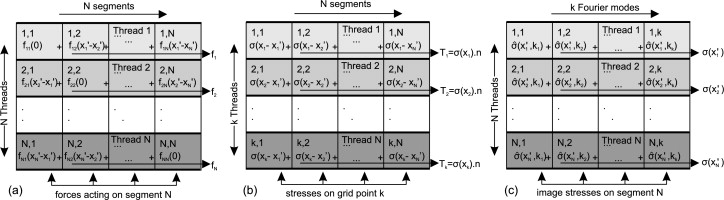
\includegraphics[width=\linewidth]{gpu_ddd.jpg}
    \caption[Parallelisation strategies for three problems in 3D DDD.]{Parallelisation strategies for: (a) the $ N^{2} $ segment interactions; (b) surface traction at k grid points and; (c) and image stresses on $ N $ segments. Image taken from \cite{gpu_ddd}.}
    \label{f:gpu_ddd}
\end{figure}

However, there is another approach \citet{gpu_ddd} did not consider. It combines both of the aforementioned strategies, $ \mathcal{O}(N^{2}) $ memory and $ \mathcal{O}(N) $ parallelisation and serialisation. Such an approach requires two copies of the input data (one per access pattern). One pattern would allow each thread to obtain its uniquely assigned segment in a coalesced manner. The second would be the serial access pattern already present. Thus obtaining the best performance possible performance at the cost of doubling the required memory. This is a better strategy provided there is enough device memory\footnote{Assuming the line direction is calculated inside the program, each dislocation line segment represents 3, 3-element vectors of type double (8-bytes per entry), totalling 72 bytes in global memory per dislocation line segment (two nodes + Burgers vector per segment). There must also be enough global memory to output the forces, which represent 1, 3-element vector of type double per dislocation node, totalling 24 bytes per node. Assuming a single dislocation loop with $ N $ nodes (therefore $ N $ segments), this brings the total global memory requirement to $ 96N $ bytes. Using two access patterns for the dislocation line segments and Burgers vector means an extra $ 72N $ bytes, giving a grand total of $ 168N $ bytes. Assuming the material parameters are stored in cosntant memory.}, if that is not so, the problem must be split into different GPU calls.

New NVidia architectures have made varying degrees of nested parallelisation possible, NVidia calls this ``dynamic parallism''. When applied to the computationally optimal solution, the $ \mathcal{O}(N^{2}) $ memory requirement is relaxed to $ \mathcal{O}(N) $ (with the same parallel-specific data structure) and $ \mathcal{O}(N^{2}) $ computational parallelism.

The parallisation strategies for the other two problems, (b) and (c) in \cref{f:gpu_ddd}, involved similar decompositions as the segment-segment interaction. For surface tractions \citet{gpu_ddd} parallelised over $ k $ surface nodes with sequential calculation and addition of the stress from each dislocation line segment. For the image stresses, they chose the reverse strategy since it allows for the serialised addition of the image stresses on dislocation line segments.

Their findings showed very promising results for parallelising DDD simulations. Compared to C, their findings showed that depending on the specific problem and parameters used, the parallel implementation reduced computational time by a factor of $ \sim 110 $ at best and $ \sim 3 $ at worst for sufficiently large problems. This is of course, provided one uses a card designed for high performance computing, as these are tailored towards double precision arithmetic and computationally intensive procedures. However, gaming graphics cards are increasingly capable of double precision arithmetic and though not as drastic, speed gains are still substantial.

\section{Project outline and new science}
\label{s:objectives}

If anything should be clear from the present work, is that materials science is far from being solved. Even within the small niche of dislocation dynamics modelling, there are a huge number of open problems and an equally large number of solutions; each with its particular sets of advantages, disadvantages, ideosyncrasies and challenges.

The rapid advancement in computer technology; pushed by the ever-increasing complexity of the problems that occupy humankind; but simultaneously restricted by the physical constraints of classical computers, have opened up new avenues for research. Research that blurs the boundaries between fields and produces something new. Undoubtedly materials science sprang up this way, when metallurgists decided to take elements from the fields of chemistry, physics and mathematics to create a new discipline.

With increasing frequency, one finds people across vastly different fields who can understand each other via a common language. The language of scientific computing, where fields intertwine and produce new research methods; where techniques developed accross disciplines are taken, improved and adapted to work on the individual researcher's problem of interest.

This project applies such techniques to accelerate and improve the ease with which outstanding problems in materials science can be tackled; making use of more accurate models, hardware acceleration and the techniques of high performance computing to enable larger and more complex simulations than ever before---striving for increasingly faithful and insightful recreations of reality with a user-friendly code on a desktop PC.

Much of the work presented herein has already proven useful in the simulation of complex simulations such as nano-indentation \cite{YU2018} and several other research projects within the Tarleton group. Here we showcase the new capabilities, findings and methods; improvements, fixes and redesign of the codebase; as well as a showcase of relatively simple, yet formerly inaccessible simulations resulting from this work. Finally, we present an ambitious proposal for future work resulting from the insights gained during the project.
\savearabiccounter

% 8772 written words.
% 7904 edited
